% Options for packages loaded elsewhere
\PassOptionsToPackage{unicode}{hyperref}
\PassOptionsToPackage{hyphens}{url}
%
\documentclass[
]{article}
\usepackage{lmodern}
\usepackage{amssymb,amsmath}
\usepackage{ifxetex,ifluatex}
\ifnum 0\ifxetex 1\fi\ifluatex 1\fi=0 % if pdftex
  \usepackage[T1]{fontenc}
  \usepackage[utf8]{inputenc}
  \usepackage{textcomp} % provide euro and other symbols
\else % if luatex or xetex
  \usepackage{unicode-math}
  \defaultfontfeatures{Scale=MatchLowercase}
  \defaultfontfeatures[\rmfamily]{Ligatures=TeX,Scale=1}
\fi
% Use upquote if available, for straight quotes in verbatim environments
\IfFileExists{upquote.sty}{\usepackage{upquote}}{}
\IfFileExists{microtype.sty}{% use microtype if available
  \usepackage[]{microtype}
  \UseMicrotypeSet[protrusion]{basicmath} % disable protrusion for tt fonts
}{}
\makeatletter
\@ifundefined{KOMAClassName}{% if non-KOMA class
  \IfFileExists{parskip.sty}{%
    \usepackage{parskip}
  }{% else
    \setlength{\parindent}{0pt}
    \setlength{\parskip}{6pt plus 2pt minus 1pt}}
}{% if KOMA class
  \KOMAoptions{parskip=half}}
\makeatother
\usepackage{xcolor}
\IfFileExists{xurl.sty}{\usepackage{xurl}}{} % add URL line breaks if available
\IfFileExists{bookmark.sty}{\usepackage{bookmark}}{\usepackage{hyperref}}
\hypersetup{
  pdftitle={SecAssignment},
  hidelinks,
  pdfcreator={LaTeX via pandoc}}
\urlstyle{same} % disable monospaced font for URLs
\usepackage{listings}
\newcommand{\passthrough}[1]{#1}
\lstset{defaultdialect=[5.3]Lua}
\lstset{defaultdialect=[x86masm]Assembler}
\usepackage{graphicx,grffile}
\makeatletter
\def\maxwidth{\ifdim\Gin@nat@width>\linewidth\linewidth\else\Gin@nat@width\fi}
\def\maxheight{\ifdim\Gin@nat@height>\textheight\textheight\else\Gin@nat@height\fi}
\makeatother
% Scale images if necessary, so that they will not overflow the page
% margins by default, and it is still possible to overwrite the defaults
% using explicit options in \includegraphics[width, height, ...]{}
\setkeys{Gin}{width=\maxwidth,height=\maxheight,keepaspectratio}
% Set default figure placement to htbp
\makeatletter
\def\fps@figure{htbp}
\makeatother
\setlength{\emergencystretch}{3em} % prevent overfull lines
\providecommand{\tightlist}{%
  \setlength{\itemsep}{0pt}\setlength{\parskip}{0pt}}
\setcounter{secnumdepth}{-\maxdimen} % remove section numbering

\title{SecAssignment}
\date{}








%Packages ------------------------------------

\usepackage{amsmath, amssymb, amsthm}
\usepackage[utf8]{inputenc}
%\usepackage[framemethod=tikz]{mdframed}
\usepackage{graphicx}
%\usetikzlibrary{calc}
%\usepackage{chngcntr}
\usepackage[T1]{fontenc}
%\usepackage{extsizes} % More Font Sizes
\usepackage[utf8]{inputenc}
\usepackage{pdfpages}
\usepackage{amsmath}
\usepackage{sectsty} %Need it for underlining Sections
\usepackage{listings}
\usepackage{lmodern}
\usepackage{amssymb,amsmath}
\usepackage{enumitem}
\usepackage{ifxetex,ifluatex}
\usepackage{lipsum}
\usepackage[T1]{fontenc}
\usepackage[utf8]{inputenc}
\usepackage[margin=1in]{geometry}

\addtolength{\skip\footins}{2pc plus 5pt} %Add whitespace before footnotes`
%\usepackage[svgnames, x11names, dvipsnames]{xcolor} %This is included with mdframed
%\usepackage{tgadventor}
%\usepackage{titlesec} % Section Colours




%Hyperlinks-----------------------------------
\usepackage{hyperref}
\hypersetup{
	colorlinks,
	citecolor=black,
	filecolor=black,
	linkcolor=black,
	urlcolor=black,
	colorlinks=true, %set true if you want colored links
	linktoc=all     %set to all if you want both sections and subsections linked
}

%Remove Section Numbers----------------
\makeatletter
\renewcommand{\@seccntformat}[1]{}
\makeatother

%Change the Font------------------------------
%\usepackage{PoiretOne}
\renewcommand*\familydefault{\sfdefault} %% Only if the base font of the document is to be sans serif

% Add rule after sections ------------------------------
\usepackage{titlesec}






%Listings----------------------------------------


\definecolor{dkgreen}{rgb}{0,0.6,0}
\definecolor{gray}{rgb}{0.5,0.5,0.5}
\definecolor{mauve}{rgb}{0.58,0,0.82}
\lstset{
	%  frame=tb,
	frame=leftline,
	framesep=15pt,
	language=,
	aboveskip=15pt,
	belowskip=20pt,
	showstringspaces=false,
	columns=flexible,
	basicstyle={\small\ttfamily},
	numbers=none,
	%  backgroundcolor=\color{Snow2},
	numberstyle=\tiny\color{gray},
	keywordstyle=\color{blue},
	commentstyle=\color{dkgreen},
	stringstyle=\color{mauve},
	breaklines=true,
    inputencoding=latin1,
	breakatwhitespace=true,
	tabsize=3,
	xleftmargin=1in,
}

% Formatting----------------------------------------
\widowpenalty=1000
\clubpenalty=1000

% Problem boxes --------------------------------------

%\newtheorem*{prob}{Problem}
%\theoremstyle{working}{\cmss}
%\newtheorem*{working}{Worked Solution}
\renewcommand{\qedsymbol}{$\blacksquare$}


\newenvironment{prob}[1][Problem]{%
	\sffamily \itshape   %
}{\endproof} %\itshape for italics

\newenvironment{sol}[1][Problem]{%
	\proof[\nopunct]  %
}{\endproof}

%%%% Define Heading colours
\definecolor{colsse}{RGB}{136, 73, 143}
\definecolor{colsss}{RGB}{156, 118, 160}
\definecolor{colspg}{RGB}{218, 168, 224}
\definecolor{coltit}{RGB}{84, 65, 86}
\definecolor{colname}{RGB}{236, 66 ,255}
% Font

% Numbering



\renewcommand{\thesection}{}
\renewcommand{\thesubsection}{}








%\renewenvironment{proof}{{\bfseries \fontfamily{ccr} \selectfont Proof}}{*something*}



\title{\color{coltit} \Huge Introduction to Data Science }
\author{Ryan Greenup ; 1780-5315}






















\begin{document}
	
	% Change Section Colour
\titleformat{\section}
{\color{colsse}\normalfont\LARGE\bfseries}
{\color{colsse}\thesection}{-1em}{}
\fontfamily{cmss}\selectfont

%SubSection
\titleformat{\subsection}
{\color{colsss}\normalfont\Large\bfseries}
{\color{colsss}\thesubsection}{-1em}{}[\rule{4 in}{2pt}]
\fontfamily{cmss}\selectfont
% Change Font
\fontfamily{cmss}\selectfont



%Paragraph
\titleformat{\paragraph}
{\color{colsss}\normalfont\large}
{\color{colsss}\theparagraph}{9em}{}[\rule{2 in}{1 pt}]
\fontfamily{cmss}\selectfont
% Change Font
\fontfamily{cmss}\selectfont



\maketitle
\tableofcontents

\newpage
	
	
	
	


\hypertarget{question-1}{%
\section{Question 1}\label{question-1}}

\hypertarget{explore-the-data-set}{%
\subsection{(1) Explore the Data Set}\label{explore-the-data-set}}
%
%\emph{\begin{quote}
% Explore the given dataset and identify the attributes of CPU that have
%linear association with CPU performance.
%\end{quote}}

Load and inspect the dataset in R:

\begin{lstlisting}[language=R]
cpu <- read.csv(file = "./Code/Datasets/CPU.csv", header = TRUE, sep = ",")
head(cpu)
\end{lstlisting}

\begin{lstlisting}
##   CycleTime MinimumMainMemory MaximumMainMemory CacheSize
## 1       125               256              6000       256
## 2        29              8000             32000        32
## 3        29              8000             32000        32
## 4        29              8000             32000        32
## 5        29              8000             16000        32
## 6        26              8000             32000        64
##   MinimumNumberOfChannels MaximumNumberOfChannels Performance
## 1                      16                     128         198
## 2                       8                      32         269
## 3                       8                      32         220
## 4                       8                      32         172
## 5                       8                      16         132
## 6                       8                      32         318
\end{lstlisting}

\begin{lstlisting}[language=R]
str(cpu)
\end{lstlisting}

\begin{lstlisting}
## 'data.frame':    209 obs. of  7 variables:
##  $ CycleTime              : int  125 29 29 29 29 26 23 23 23 23 ...
##  $ MinimumMainMemory      : int  256 8000 8000 8000 8000 8000 16000 16000 16000 32000 ...
##  $ MaximumMainMemory      : int  6000 32000 32000 32000 16000 32000 32000 32000 64000 64000 ...
##  $ CacheSize              : int  256 32 32 32 32 64 64 64 64 128 ...
##  $ MinimumNumberOfChannels: int  16 8 8 8 8 8 16 16 16 32 ...
##  $ MaximumNumberOfChannels: int  128 32 32 32 16 32 32 32 32 64 ...
##  $ Performance            : int  198 269 220 172 132 318 367 489 636 1144 ...
\end{lstlisting}

\begin{lstlisting}[language=R]
#dim(cpu)
#summary(cpu)
\end{lstlisting}

From the output it can be seen that this is a data set containing 6
predictive features corresponding to 1 ouput variable with 209
observations.

\hypertarget{identify-any-linear-relations}{%
\subsubsection{Identify any Linear
Relations}\label{identify-any-linear-relations}}

In order to identify any linear relations
\passthrough{\lstinline!corrplot()!} may be used to consider the
strength and direction of any linear correlation between variables:

\begin{lstlisting}[language=R]
cpu_pretty <- cpu
names(cpu_pretty) <- c("Cycle\nPeriod", "Min\nMemory", "Max\nMemory", "Cache", "Min\nChannels", "Max\nChannels", "Performance")

corrplot(cor(cpu_pretty),method = 'ellipse', type = 'upper')
\end{lstlisting}

\begin{figure}
\centering
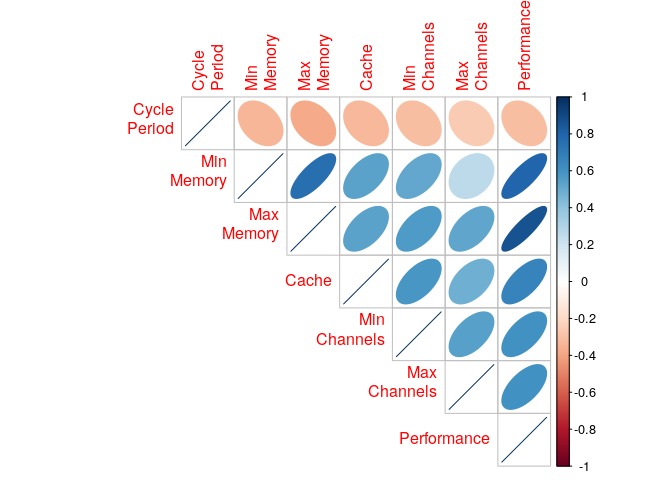
\includegraphics[width=0.7\linewidth]{SecAssignment_files/figure-html/corrplot-1.png}
\caption{Correlation Matrix for CPU Characteristics}
\label{corrplot}
\end{figure}



This suggests that the Maximum Main memory has a strong positive
correlation with performance. In order to further assess the
relationship between performance and maximum main memory a scatter plot
will be drawn in order to investigate the relationships, the
\passthrough{\lstinline!pairs()!} function is not ideal here because we
only need to consider \emph{Performance} as a response.

It would be possible to call a loop over various plots using the base
packages but it would be more appropriate to create a \emph{tidy} data
frame and plot multiple facets using
\passthrough{\lstinline!ggplot2()!}:

\begin{lstlisting}[language=R]
# layout(matrix(1:6, nrow = 2))
# for (i in 1:6) {
# plot(y=cpu$Performance, x = cpu[,i], xlab = names(cpu)[i], ylab = "Performance")
# }


  # New facet label names for supp variable
pred.labs <- c("Max\nMemory", "Min\nMemory")
names(pred.labs) <- c("MaximumMainMemory", "MinimumMainMemory")


# Create the plot
# p + facet_grid(
#   dose ~ supp, 
#   labeller = labeller(dose = dose.labs, supp = supp.labs)
#   )

subset <- names(cpu_pretty)[2:3]
cpu.tidymem <- pivot_longer(data = cpu_pretty[,c("Performance",subset)], cols = subset )
pmem <- ggplot(cpu.tidymem, aes(x = value, y = Performance, col = name)) +
  geom_point() + 
  theme_bw() +
  geom_smooth(method = 'lm')+
  facet_grid(. ~ name ) +
  labs(col = "CPU \n Characteristic", x = NULL)


cpu.else <- dplyr::select(cpu_pretty, -subset)
cpu.tidyelse <- pivot_longer(data = cpu.else, cols = 1:(-1+length(cpu.else)))
pelse <- ggplot(cpu.tidyelse, aes(x = value, y = Performance, col = name)) +
  geom_point() + 
  theme_bw() +
  geom_smooth(method = 'lm')+
  facet_grid(. ~ name, scales = "free_x") + 
  labs(col = "CPU \n Characteristic", x = NULL)

grid.arrange(pmem, pelse, nrow = 2)
\end{lstlisting}



\begin{figure}
\centering
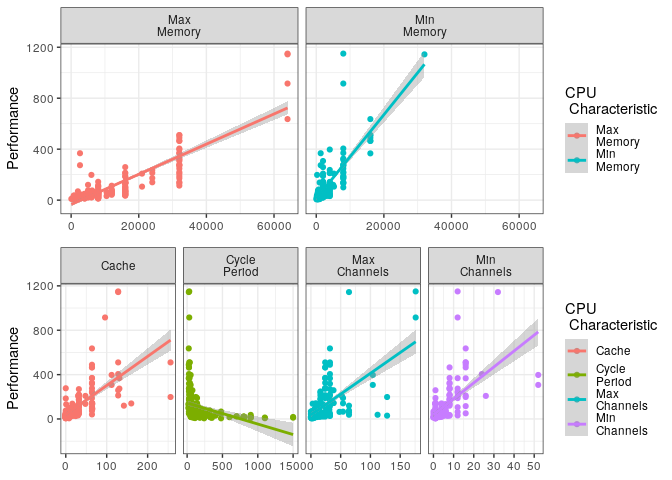
\includegraphics[width=0.7\linewidth]{SecAssignment_files/figure-html/sp-1.png} 
\caption{Scatter Plots of Perfomance given CPU Characteristics}
\label{sp-1}
\end{figure}


The preceeding code produces the plot shown in Figure \ref{sp-1}, from which it may be seen that all of the variables, with the exception of
\passthrough{\lstinline!CycleTime!}, are linearly correlated with
performance, however the plots demonstrate a violation of the
assumption of homoskedasticity.

\hypertarget{select-the-most-suitable-attribute-to-use-for-simple-linear-regression}{%
\subsection{(2) Select the most Suitable Attribute to use for Simple
Linear
Regression}\label{select-the-most-suitable-attribute-to-use-for-simple-linear-regression}}

Many of the variables are linearly correlated with performance, however,
as mentioned, the plots violate the assumption of homoskedasticity, for
this reason a \(\log\) transform is used.

The cycle period appears to be inversely proportional to performance, it
seems reasonable that cycle frequency will be proportional to
performance and for this reason a linear model of cycle frequency
(an inverse transform), will be considered as a potential attribute for
Simple Linear Regression.

The variables \passthrough{\lstinline!MaximumMainMemory!} and
\passthrough{\lstinline!MinimimMainMemory!} are strongly correlated
predictors and so only one of the two should be considered as a
predictive feature. It can be seen from the correlation matrix that
\passthrough{\lstinline!MaximumMainMemory!} is more strongly correlated
with performance and so it is chosen as the potential predictive
feature.

\begin{lstlisting}[language=R]
# layout(matrix(1:6, nrow = 2))
# for (i in 1:6) {
# plot(y=cpu$Performance, x = cpu[,i], xlab = names(cpu)[i], ylab = "Performance")
# }

cpu_pretty$"ln(Performance)" <- log(cpu_pretty$Performance)
# names(cpu_pretty)[7] <- "ln(Performance)"



subset <- names(cpu_pretty)[2]
cpu.tidymem <- pivot_longer(data = cpu_pretty[,c("ln(Performance)",subset)], cols = subset )
pmem <- ggplot(cpu.tidymem, aes(x = value, y = `ln(Performance)`, col = name)) +
  geom_point() + 
  theme_bw() +
  geom_smooth(method = 'lm')+
  facet_grid(. ~ name ) +
  labs(col = "CPU \n Characteristic", x = NULL)


cpu.else <- dplyr::select(cpu_pretty, -subset)
cpu.tidyelse <- pivot_longer(data = cpu.else, cols = c(2,3,4))
pelse <- ggplot(cpu.tidyelse, aes(x = value, y = `ln(Performance)`, col = name)) +
  geom_point() + 
  theme_bw() +
  geom_smooth(method = 'lm')+
  facet_grid(. ~ name, scales = "free_x") + 
  labs(col = "CPU \n Characteristic", x = NULL)

grid.arrange(pmem, pelse, nrow = 2)
\end{lstlisting}

\begin{figure}[h!]
\centering
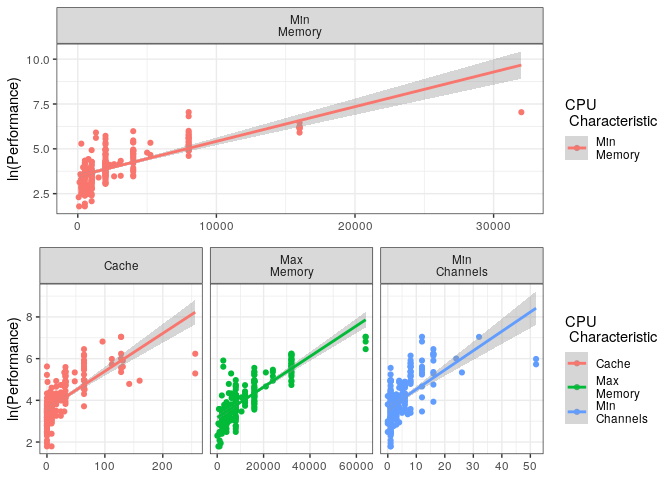
\includegraphics[width=0.7\linewidth]{SecAssignment_files/figure-html/splog-1.png}
\caption{Scatter Plot of Log-Scaled Perfomance over CPU Characteristics}
\label{splog-1}
\end{figure}

\newpage

The preceding code produces the plots shown in figure \ref{splog-1}, wherein none of these plots are linear despite the transform. It would be
inappropriate to fit a linear model to data that violates the underlying
assumptions of linear regression, instead, consider the cpu frequency:

\begin{lstlisting}[language=R]
cpu_pretty$"Root Performance" <- sqrt(cpu_pretty$Performance)
cpu_pretty$Frequency <- (1/cpu_pretty$"Cycle\nPeriod")
#
cpufreq <- dplyr::select(cpu_pretty, c("Performance", "ln(Performance)", "Frequency"))
cpuTidyfreq <- pivot_longer(data = cpufreq, cols = c("Performance", "ln(Performance)"), names_to = "Performance\nMeasure")


ggplot(data = cpuTidyfreq, aes(x = Frequency, y = value, col = `Performance\nMeasure`)) +
  geom_point() +
  theme_bw() +
  geom_smooth(method = 'lm') +
  facet_grid(`Performance\nMeasure` ~ ., scales = "free_y")
\end{lstlisting}

\begin{figure}[htbp]
	\centering
	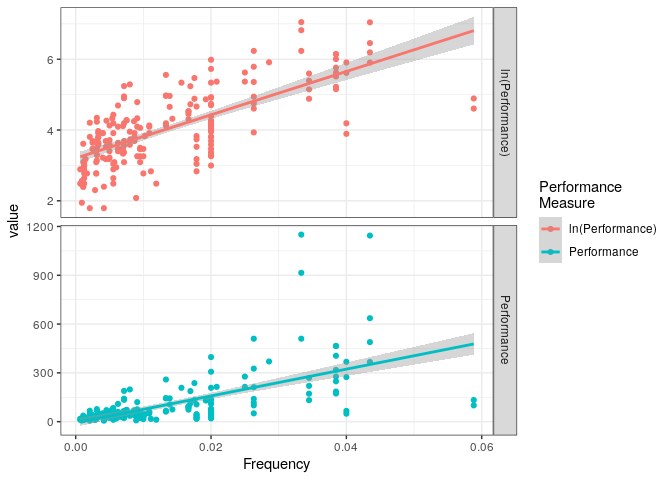
\includegraphics[width=0.7\linewidth]{SecAssignment_files/figure-html/unnamed-chunk-2-1.png}
	\caption{Scatter Plot of Log-Scaled Perfomance over CPU Frequency}
	\label{unnamed21}
\end{figure}


The preceding code produces the plots in figure \ref{unnamed21}, from this it can be seen that the frequency is far more linear than
other variables after a log transform, for this reason frequency is
chosen as the most suitable attribute from which to predict CPU
performance with simple linear regression.

Before the log transform it is too heteroskedastic and violates the
assumption of Gaussian residuals, the $\log$-transformed plot appears to have
constant variance over the frequency and performance measurments and appears to be reasonably linear, whereas other
attributes appear to follow a concave-down and non-linear trend
following the transform.

\newpage

The linear model chosen is of the form:


\begin{align}
\log{\left( Y_{Perf}\right)} = \beta_0 + \beta_1 \times X_{Freq} \label{q1ref}
\end{align}

this attribute is chosen because it is the only attribute that has a
linear relationship (albeit after a $\log$ transform) and the only
attribute that has constant variance from the model.

\hypertarget{create-the-model}{%
\subsubsection{Create the Model}\label{create-the-model}}

The model can be created using the \passthrough{\lstinline!lm!}
function, it is important to not use \passthrough{\lstinline!I(log(Y))!}
in the model call, otherwise residual plots may not be generated correctly.

\begin{lstlisting}[language=R]
# Training Split
train <- sample(nrow(cpu) * 0.45)
cpu_mod.slm <- lm(formula = `ln(Performance)` ~ Frequency, data = cpu_pretty, subset = train)
val.Error <- (cpu_pretty$`ln(Performance)`[-train] - predict(object = cpu_mod.slm, newdata = cpu_pretty[-train,]))^2 %>%
  mean() %>% 
  sqrt() %>% 
  exp() %>% 
  round(3) %>% 
  paste("is the validation RMSE (expected distance from model") %>% 
  print()
\end{lstlisting}

\begin{lstlisting}
## [1] "2.249 is the validation RMSE (expected distance from model"
\end{lstlisting}

\begin{lstlisting}[language=R]
# Return Model
cpu_mod.slm <- lm(`ln(Performance)` ~ Frequency, data = cpu_pretty, subset = NULL)
summary(cpu_mod.slm)
\end{lstlisting}

\begin{lstlisting}
## 
## Call:
## lm(formula = `ln(Performance)` ~ Frequency, data = cpu_pretty, 
##     subset = NULL)
## 
## Residuals:
##      Min       1Q   Median       3Q      Max 
## -2.20171 -0.43299  0.04276  0.48407  1.80214 
## 
## Coefficients:
##             Estimate Std. Error t value Pr(>|t|)    
## (Intercept)   3.2034     0.0769   41.66   <2e-16 ***
## Frequency    61.2591     4.2183   14.52   <2e-16 ***
## ---
## Signif. codes:  0 '***' 0.001 '**' 0.01 '*' 0.05 '.' 0.1 ' ' 1
## 
## Residual standard error: 0.7396 on 207 degrees of freedom
## Multiple R-squared:  0.5047, Adjusted R-squared:  0.5023 
## F-statistic: 210.9 on 1 and 207 DF,  p-value: < 2.2e-16
\end{lstlisting}

Which provides the specific model:

\begin{align}
\log_e\left( Y_{Perf}   \right) = 3.2034 + 61.26 \times X_{Freq} \label{q1slrpar}
\end{align}



The intercept and slope are both highly significant $p$-values, indicating
that the probability of incorrectly rejecting the null hypothesis, that
there is no linear relationship between frequency and performance
(presuming that the linear assumptions are valid, which they appear to
be), given that the other predictive features are constant, is very low.

This model is accpeted because all the coefficients are significant, and
the expected validation error is only 0.8, where as the standard
deviation of the performance variable is 160. 

The \(R\)-squared value is
quite poor (a measurement of the proportion of variance explained by the
model), which indicates that there is potentially a better model for the
data.

\newpage 

\hypertarget{model-the-performance-using-multiple-linear-regression}{%
\subsection{(3) Model the Performance using Multiple Linear
Regression}\label{model-the-performance-using-multiple-linear-regression}}

From the correlation plot at figure \ref{corrplot} it can be seen that the
following are strongly postively correlated with CPU performance:

\begin{itemize}
\tightlist
\item
  Minimum Main Memory
\item
  Maximum Main Memory
\end{itemize}

While the following are weakly correlated with CPU performance.

\begin{itemize}
\tightlist
\item
  Cache Size
\item
  Minimum Channels
\item
  Maximum Channels
\end{itemize}

Are weakly correlated with CPU performance.

\passthrough{\lstinline!Cycletime!} is very weakly negatively correlated
with performance and may not be useful predictor of performance in a linear model; however
from before it is clear that frequency is indeed a strongly correlated
predictor of performance and will hence be included in any predictive
model.

\hypertarget{collinearity}{%
\subsubsection{Collinearity}\label{collinearity}}

The minimum and maximum amount of memory appear to be strongly
positively correlated, indicating that it may be appropriate to consider
only one of those two variables in a model, similar mutlicolinearity is
observed between maximum and minimum channels.

In order to assess multi-collinearity the \emph{variance inflation
factors} (\emph{VIF}) \footnote{Refer to p.~101 of TB} will be
calculated for every term of a linear model, a VIF value that exceeds 5
indicates a problematic amount of collinearity.

\hypertarget{linearity}{%
\subsubsection{Linearity}\label{linearity}}

Although the \emph{Pearson Correlation Coefficient} measures the
strength of the linear relationship between variables, the data may have
a non-linear tendency that may compromise the model's capacity to
forecast; this can be seen from the scatter plots at figure \ref{sp-1}. 
This could potentially be overcome with a concave transform, such as a
log-transform, this will be considered after fitting the model by
analysing the residuals.

\hypertarget{feature-interaction}{%
\subsubsection{Feature Interaction}\label{feature-interaction}}

A CPU with a higher frequency (i.e.~a lower value for
\passthrough{\lstinline!CycleTime!}) may benefit more significantly from
more memory and more channels, hence we will consider the following
interaction terms in a mulitple linear regression:

\begin{itemize}
\tightlist
\item
  Max Memory and Frequency
\item
  Max Channels and Frequency
\item
  Max Channels, Max Memory and Frequency.
\end{itemize}

\hypertarget{fit-the-model}{%
\subsubsection{Fit the Model}\label{fit-the-model}}

Backward elimination will be implemented in order to choose the model.

\begin{lstlisting}[language=R]
cpu$Frequency <- cpu$CycleTime^-1
cpu_mod.mlm <- lm(Performance ~ . -CycleTime + I(MaximumNumberOfChannels * MaximumMainMemory * Frequency)  + I(MaximumNumberOfChannels * Frequency) + I( MaximumMainMemory * Frequency)   , data = cpu)
summary(cpu_mod.mlm)
\end{lstlisting}

\begin{lstlisting}[basicstyle=\scriptsize \ttfamily]
# Call:
#   lm(formula = Performance ~ . - CycleTime + I(MaximumNumberOfChannels * 
#                                                  MaximumMainMemory * Frequency) + I(MaximumNumberOfChannels * 
#                                                                                       Frequency) + I(MaximumMainMemory * Frequency), data = cpu)
# 
# Residuals:
#   Min       1Q   Median       3Q      Max 
# -148.536  -12.912   -0.918   12.896  213.929 
# 
# Coefficients:
#   Estimate Std. Error t value Pr(>|t|)    
# (Intercept)                                                 1.194e+01  6.686e+00   1.785   0.0757 .  
# MinimumMainMemory                                           1.327e-02  1.521e-03   8.722 1.09e-15 ***
#   MaximumMainMemory                                           1.602e-03  6.262e-04   2.559   0.0113 *  
#   CacheSize                                                   7.876e-01  9.486e-02   8.303 1.54e-14 ***
#   MinimumNumberOfChannels                                     4.696e-01  6.948e-01   0.676   0.5000    
# MaximumNumberOfChannels                                    -5.654e-01  2.601e-01  -2.174   0.0309 *  
#   Frequency                                                  -1.373e+03  5.747e+02  -2.389   0.0178 *  
#   I(MaximumNumberOfChannels * MaximumMainMemory * Frequency)  9.272e-04  4.511e-04   2.056   0.0411 *  
#   I(MaximumNumberOfChannels * Frequency)                      7.703e+01  3.428e+01   2.247   0.0257 *  
#   I(MaximumMainMemory * Frequency)                            3.776e-02  2.657e-02   1.421   0.1568    
# ---
#   Signif. codes:  0 '***' 0.001 '**' 0.01 '*' 0.05 '.' 0.1  '' 1
# 
# Residual standard error: 38.7 on 199 degrees of freedom
# Multiple R-squared:  0.9446,	Adjusted R-squared:  0.9421 
# F-statistic:   377 on 9 and 199 DF,  p-value: < 2.2e-16
\end{lstlisting}

The least significant predictor is the variable
\passthrough{\lstinline!MinimimMainMemory!}, this could be explained by
intercorrelation between terms. Before proceeding the \emph{variable
inflation factor} will be considered, this can be acheived by using the
\passthrough{\lstinline!car::vif()!} function on a model.

\begin{lstlisting}[language=R]
library(car)
vif(cpu_mod.mlm)
\end{lstlisting}

\begin{lstlisting}
##                                          MinimumMainMemory 
##                                                   4.836088 
##                                          MaximumMainMemory 
##                                                   7.488001 
##                                                  CacheSize 
##                                                   2.062585 
##                                    MinimumNumberOfChannels 
##                                                   3.115217 
##                                    MaximumNumberOfChannels 
##                                                   6.350779 
##                                                  Frequency 
##                                                   6.779859 
## I(MaximumNumberOfChannels * MaximumMainMemory * Frequency) 
##                                                  44.904601 
##                     I(MaximumNumberOfChannels * Frequency) 
##                                                  75.619039 
##                           I(MaximumMainMemory * Frequency) 
##                                                  19.576037
\end{lstlisting}

Typically a VIF above 10 indicates a problematic amount of colinearity,
before we may commence with backwards elimination it will be necessary
to remove colinear interaction factors and then consider combining
remaining colinear factors into combined predictor.

The Interaction term of channels and frequency has the highest VIF so it
will be removed first:

\begin{lstlisting}[language=R]
cpu_mod.mlm <- lm(Performance ~ . -CycleTime + I(MaximumNumberOfChannels * MaximumMainMemory * Frequency) + I( MaximumMainMemory * Frequency)   , data = cpu) 
vif(cpu_mod.mlm)
\end{lstlisting}

\begin{lstlisting}
##                                          MinimumMainMemory 
##                                                   4.834693 
##                                          MaximumMainMemory 
##                                                   7.295421 
##                                                  CacheSize 
##                                                   1.996105 
##                                    MinimumNumberOfChannels 
##                                                   2.092357 
##                                    MaximumNumberOfChannels 
##                                                   2.865647 
##                                                  Frequency 
##                                                   3.498502 
## I(MaximumNumberOfChannels * MaximumMainMemory * Frequency) 
##                                                   4.333099 
##                           I(MaximumMainMemory * Frequency) 
##                                                  19.421320
\end{lstlisting}


The interaction term of \passthrough{\lstinline!MaximumMainMemory!} and
\passthrough{\lstinline!Frequency!} has too high a
\passthrough{\lstinline!VIF()!} factor, so that will be removed:

\begin{lstlisting}[language=R]
cpu_mod.mlm <- lm(Performance ~ . -CycleTime + I(MaximumNumberOfChannels * MaximumMainMemory * Frequency)  , data = cpu) 
vif(cpu_mod.mlm)
\end{lstlisting}

\begin{lstlisting}
##                                          MinimumMainMemory 
##                                                   3.169999 
##                                          MaximumMainMemory 
##                                                   4.302255 
##                                                  CacheSize 
##                                                   1.897146 
##                                    MinimumNumberOfChannels 
##                                                   2.074288 
##                                    MaximumNumberOfChannels 
##                                                   2.773799 
##                                                  Frequency 
##                                                   2.226321 
## I(MaximumNumberOfChannels * MaximumMainMemory * Frequency) 
##                                                   2.931035
\end{lstlisting}


The VIF factors are sufficiently low, despite the correlation between
maximum and minimum memory, the sufficiently low VIF values indicate
that there is iinsufficient evidence to remove minimum memory on the
grounds of colinearity and the term will not be removed.

A VIF factor of 4 is still somewhat high, however it would be
inappropriate to exclude either variable because having a low minimum
memory is qualitatively different from having a low maximum memory, a
poor configuration of CPU is indicative poor performance and hence the
variables should remain unaltered.

\begin{lstlisting}[language=R]
cpu_mod.mlm %>% summary()
\end{lstlisting}

\begin{lstlisting}
## 
## Call:
## lm(formula = Performance ~ . - CycleTime + I(MaximumNumberOfChannels * 
##     MaximumMainMemory * Frequency), data = cpu)
## 
## Residuals:
##      Min       1Q   Median       3Q      Max 
## -158.832  -11.365   -1.345   13.350  226.565 
## 
## Coefficients:
##                                                              Estimate
## (Intercept)                                                 1.689e+00
## MinimumMainMemory                                           1.431e-02
## MaximumMainMemory                                           1.862e-03
## CacheSize                                                   8.004e-01
## MinimumNumberOfChannels                                     1.429e+00
## MaximumNumberOfChannels                                    -1.708e-01
## Frequency                                                  -1.693e+02
## I(MaximumNumberOfChannels * MaximumMainMemory * Frequency)  1.988e-03
##                                                            Std. Error
## (Intercept)                                                 4.944e+00
## MinimumMainMemory                                           1.246e-03
## MaximumMainMemory                                           4.800e-04
## CacheSize                                                   9.200e-02
## MinimumNumberOfChannels                                     5.734e-01
## MaximumNumberOfChannels                                     1.738e-01
## Frequency                                                   3.331e+02
## I(MaximumNumberOfChannels * MaximumMainMemory * Frequency)  1.165e-04
##                                                            t value
## (Intercept)                                                  0.342
## MinimumMainMemory                                           11.485
## MaximumMainMemory                                            3.879
## CacheSize                                                    8.700
## MinimumNumberOfChannels                                      2.492
## MaximumNumberOfChannels                                     -0.983
## Frequency                                                   -0.508
## I(MaximumNumberOfChannels * MaximumMainMemory * Frequency)  17.062
##                                                            Pr(>|t|)    
## (Intercept)                                                0.733031    
## MinimumMainMemory                                           < 2e-16 ***
## MaximumMainMemory                                          0.000142 ***
## CacheSize                                                  1.19e-15 ***
## MinimumNumberOfChannels                                    0.013498 *  
## MaximumNumberOfChannels                                    0.326994    
## Frequency                                                  0.611711    
## I(MaximumNumberOfChannels * MaximumMainMemory * Frequency)  < 2e-16 ***
## ---
## Signif. codes:  0 '***' 0.001 '**' 0.01 '*' 0.05 '.' 0.1 ' ' 1
## 
## Residual standard error: 39.14 on 201 degrees of freedom
## Multiple R-squared:  0.9428, Adjusted R-squared:  0.9408 
## F-statistic: 473.1 on 7 and 201 DF,  p-value: < 2.2e-16
\end{lstlisting}

The term \passthrough{\lstinline!Frequency!} is not significant and so
it will be removed from the model:

\begin{lstlisting}[language=R]
cpu_mod.mlm <- lm(Performance ~ . -Frequency -CycleTime + I(MaximumNumberOfChannels * MaximumMainMemory * Frequency)  , data = cpu) 
#vif(cpu_mod.mlm)
 summary(cpu_mod.mlm)
\end{lstlisting}

\begin{lstlisting}
## 
## Call:
## lm(formula = Performance ~ . - Frequency - CycleTime + I(MaximumNumberOfChannels * 
##     MaximumMainMemory * Frequency), data = cpu)
## 
## Residuals:
##     Min      1Q  Median      3Q     Max 
## -158.42  -11.51   -1.13   14.02  222.10 
## 
## Coefficients:
##                                                              Estimate
## (Intercept)                                                 0.7551310
## MinimumMainMemory                                           0.0141224
## MaximumMainMemory                                           0.0018003
## CacheSize                                                   0.7946907
## MinimumNumberOfChannels                                     1.3862559
## MaximumNumberOfChannels                                    -0.1589160
## I(MaximumNumberOfChannels * MaximumMainMemory * Frequency)  0.0019897
##                                                            Std. Error
## (Intercept)                                                 4.5817350
## MinimumMainMemory                                           0.0011895
## MaximumMainMemory                                           0.0004635
## CacheSize                                                   0.0911478
## MinimumNumberOfChannels                                     0.5661210
## MaximumNumberOfChannels                                     0.1719460
## I(MaximumNumberOfChannels * MaximumMainMemory * Frequency)  0.0001163
##                                                            t value
## (Intercept)                                                  0.165
## MinimumMainMemory                                           11.873
## MaximumMainMemory                                            3.884
## CacheSize                                                    8.719
## MinimumNumberOfChannels                                      2.449
## MaximumNumberOfChannels                                     -0.924
## I(MaximumNumberOfChannels * MaximumMainMemory * Frequency)  17.109
##                                                            Pr(>|t|)    
## (Intercept)                                                0.869256    
## MinimumMainMemory                                           < 2e-16 ***
## MaximumMainMemory                                          0.000139 ***
## CacheSize                                                  1.03e-15 ***
## MinimumNumberOfChannels                                    0.015190 *  
## MaximumNumberOfChannels                                    0.356474    
## I(MaximumNumberOfChannels * MaximumMainMemory * Frequency)  < 2e-16 ***
## ---
## Signif. codes:  0 '***' 0.001 '**' 0.01 '*' 0.05 '.' 0.1 ' ' 1
## 
## Residual standard error: 39.07 on 202 degrees of freedom
## Multiple R-squared:  0.9427, Adjusted R-squared:  0.941 
## F-statistic: 553.9 on 6 and 202 DF,  p-value: < 2.2e-16
\end{lstlisting}

The term \passthrough{\lstinline!MaximumNumberOfChannels!} is not
significant and so it will be removed from the model:

\begin{lstlisting}[language=R]
cpu_mod.mlm <- lm(Performance ~ . -MaximumNumberOfChannels -Frequency -CycleTime + I(MaximumNumberOfChannels * MaximumMainMemory * Frequency)  , data = cpu) 
#vif(cpu_mod.mlm)
 summary(cpu_mod.mlm)
\end{lstlisting}

\begin{lstlisting}
## 
## Call:
## lm(formula = Performance ~ . - MaximumNumberOfChannels - Frequency - 
##     CycleTime + I(MaximumNumberOfChannels * MaximumMainMemory * 
##     Frequency), data = cpu)
## 
## Residuals:
##      Min       1Q   Median       3Q      Max 
## -155.673  -11.509   -0.239   13.303  224.823 
## 
## Coefficients:
##                                                              Estimate
## (Intercept)                                                -7.778e-01
## MinimumMainMemory                                           1.449e-02
## MaximumMainMemory                                           1.770e-03
## CacheSize                                                   7.722e-01
## MinimumNumberOfChannels                                     1.193e+00
## I(MaximumNumberOfChannels * MaximumMainMemory * Frequency)  1.930e-03
##                                                            Std. Error
## (Intercept)                                                 4.269e+00
## MinimumMainMemory                                           1.122e-03
## MaximumMainMemory                                           4.621e-04
## CacheSize                                                   8.782e-02
## MinimumNumberOfChannels                                     5.261e-01
## I(MaximumNumberOfChannels * MaximumMainMemory * Frequency)  9.685e-05
##                                                            t value
## (Intercept)                                                 -0.182
## MinimumMainMemory                                           12.913
## MaximumMainMemory                                            3.829
## CacheSize                                                    8.793
## MinimumNumberOfChannels                                      2.269
## I(MaximumNumberOfChannels * MaximumMainMemory * Frequency)  19.930
##                                                            Pr(>|t|)    
## (Intercept)                                                0.855630    
## MinimumMainMemory                                           < 2e-16 ***
## MaximumMainMemory                                          0.000171 ***
## CacheSize                                                  6.24e-16 ***
## MinimumNumberOfChannels                                    0.024350 *  
## I(MaximumNumberOfChannels * MaximumMainMemory * Frequency)  < 2e-16 ***
## ---
## Signif. codes:  0 '***' 0.001 '**' 0.01 '*' 0.05 '.' 0.1 ' ' 1
## 
## Residual standard error: 39.05 on 203 degrees of freedom
## Multiple R-squared:  0.9425, Adjusted R-squared:  0.941 
## F-statistic:   665 on 5 and 203 DF,  p-value: < 2.2e-16
\end{lstlisting}

All Model terms are now significant so the model is accepted as a
potential model.

\hypertarget{find-the-best-model}{%
\subsubsection{Find the Best Model}\label{find-the-best-model}}

Backward elimination will not necessarily return the optimal model,
instead the method of \emph{best subset selection} should be used, which
involves choosing the best variables corresponding to a given model size
by way of the training error and then determining the best model size
using an adjusted-measurement of training error, 10-fold
cross-validation could also be used, however there exists the
possibility that no single model performs significantly better and it
would be more appropriate to instead consider using lasso regression,
this is outside the scope of this work and so instead the simplest model
that performs the best with respect to adjusted training error
measurements will be accepted.

\hypertarget{use-the-best-subset-selection}{%
\paragraph{Use the best subset
selection}\label{use-the-best-subset-selection}}

\textit{Best Subset Selection} may be implemented by using the \verb|regsubsets()| function:

\begin{lstlisting}[language=R]
allMLM <- regsubsets(Performance ~ . -CycleTime, cpu)
allMLMSum <- summary(allMLM)
\end{lstlisting}

Now take the the AIC, BIC and adjusted R-squared values as an estimate
of the model error

\begin{lstlisting}[language=R]
ErrorCrit <- tibble("preds" = (1:(ncol(cpu)-2)), "adjrsq" = allMLMSum$adjr2, "bic" = allMLMSum$bic, "cp"= allMLMSum$cp)
ErrorCritSTD <- ErrorCrit
ErrorCritSTD$adjrsq <- -(ErrorCritSTD$adjrsq-mean(ErrorCritSTD$adjrsq))/sd(ErrorCritSTD$adjrsq)
ErrorCritSTD$bic <- (ErrorCritSTD$bic-mean(ErrorCritSTD$bic))/sd(ErrorCritSTD$bic)
ErrorCritSTD$cp <- (ErrorCritSTD$cp-mean(ErrorCritSTD$cp))/sd(ErrorCritSTD$cp)


allMLMSum$adjr2
\end{lstlisting}

\begin{lstlisting}
## [1] 0.7435259 0.7981760 0.8444189 0.8567846 0.8563690 0.8557426
\end{lstlisting}

\begin{lstlisting}[language=R]
ErrorCrit.tidy <- pivot_longer(data = ErrorCrit, cols = c(adjrsq, bic, cp), names_to = "adjTrError")
ErrorCrit.tidy <- pivot_longer(data = ErrorCritSTD, cols = c(adjrsq, bic, cp), names_to = "adjTrError")



ErrorCrit.tidy$adjTrError[ErrorCrit.tidy$adjTrError=="adjrsq"] <- "Adjusted R-Squared"
ErrorCrit.tidy$adjTrError[ErrorCrit.tidy$adjTrError=="bic"] <- "BIC"
ErrorCrit.tidy$adjTrError[ErrorCrit.tidy$adjTrError=="cp"] <- "Cp"

ggplot(ErrorCrit.tidy, aes(x= preds, y = value, col = adjTrError)) + 
  geom_point(size = 4) +
  geom_line() + 
  labs(x = "Number of Predictors" , y = "Standardised Training RSS" , col = "Adjusted Training Error", title = "Model Performance Given Parameters") +
  theme_classic() +
  geom_vline(xintercept = which.min(allMLMSum$bic), col = "IndianRed")
\end{lstlisting}



\begin{figure}
	\centering
	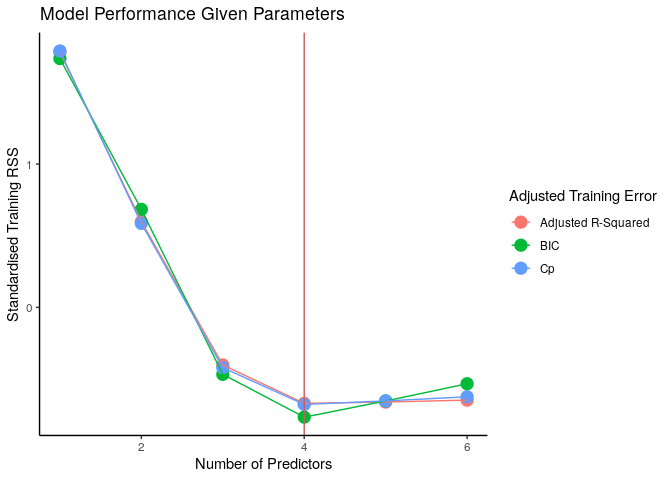
\includegraphics[width=0.7\linewidth]{SecAssignment_files/figure-html/unnamed-chunk-13-1.png}
	\caption{Model performance as determined by the number of predictors using adjusted training errors to estimate testing error, the RSS values are standardised so the adjusted training errors may be compared.}
	\label{bestsubsetError}
\end{figure}



The preceding code produces the plot in figure \ref{bestsubsetError} which demonstrates that the best performing linear regression is the
model with 4 predictors, the predictors being as shown in equation \eqref{MultMod}:

\begin{lstlisting}[language=R]
coef(allMLM, 4) %>% signif(2)
\end{lstlisting}

\begin{lstlisting}
##             (Intercept)       MinimumMainMemory       MaximumMainMemory 
##                -41.0000                  0.0150                  0.0053 
##               CacheSize MaximumNumberOfChannels 
##                  0.5900                  1.4000
\end{lstlisting}

and hence the model would be:

\begin{lstlisting}[language=R]
best.Mod.mlm <- lm(Performance ~ MinimumMainMemory + MaximumMainMemory + CacheSize + MaximumNumberOfChannels, cpu)
summary(best.Mod.mlm)
\end{lstlisting}

\begin{lstlisting}
## 
## Call:
## lm(formula = Performance ~ MinimumMainMemory + MaximumMainMemory + 
##     CacheSize + MaximumNumberOfChannels, data = cpu)
## 
## Residuals:
##     Min      1Q  Median      3Q     Max 
## -186.73  -26.08    8.27   26.99  402.87 
## 
## Coefficients:
##                           Estimate Std. Error t value Pr(>|t|)    
## (Intercept)             -40.982864   6.041898  -6.783 1.25e-10 ***
## MinimumMainMemory         0.014887   0.001815   8.202 2.61e-14 ***
## MaximumMainMemory         0.005330   0.000645   8.263 1.79e-14 ***
## CacheSize                 0.587097   0.135764   4.324 2.39e-05 ***
## MaximumNumberOfChannels   1.436179   0.210954   6.808 1.08e-10 ***
## ---
## Signif. codes:  0 '***' 0.001 '**' 0.01 '*' 0.05 '.' 0.1 ' ' 1
## 
## Residual standard error: 60.86 on 204 degrees of freedom
## Multiple R-squared:  0.8595, Adjusted R-squared:  0.8568 
## F-statistic: 312.1 on 4 and 204 DF,  p-value: < 2.2e-16
\end{lstlisting}

\begin{align}
Y_{\textsf{Perf}} = -40 + 0.015\times \textsf{MinMem}  + 0.0053 \times \textsf{MaxMem} + 0.59\times \textsf{Cache} + 1.4\times \textsf{MaxChannels} \label{MultMod}
\end{align}

Despite the high performance of frequency for simple linear regression,
suprisingly, it is not a factor in the model; moreover, despite the
anticipated correlation between minimum memory and maximum memory both are factors in the best performing model. 
%Next the interaction between memory and frequency will be considered  to see if that is a non-colinear and significant term.

\hypertarget{consider-interaction-terms}{%
\subsubsection{Consider Interaction
Terms}\label{consider-interaction-terms}}

We may now wish to consider the interaction term frequency and memory,
as it stands to reason that higher memory may offer more performance for
a CPU that has a higher frequency, moreover the three way interaction
term was significant previously and so an interaction term will by
considered:

\begin{lstlisting}[language=R]
Int.Mod <- lm(Performance ~ -CycleTime + MinimumMainMemory + MaximumMainMemory + CacheSize + MaximumNumberOfChannels + MaximumMainMemory:Frequency:MaximumNumberOfChannels, data = cpu)

#vif(Int.Mod)
newBIC <- (Int.Mod) %>% BIC()
origBIC <- summary(regsubsets(Performance ~ . -CycleTime, cpu))$bic[4]
\end{lstlisting}

The preceding code provides that adding the interaction term increased the adjusted training error from
-384 to 2162 and hence this interaction term is rejected
on the grounds that it does not improve the model performance on unseen
data as predicted by the BIC value.

Hence the accepted optimal linear model remains unchanged as shown in equation \eqref{MultMod} .

\hypertarget{d-model-diagnostics}{%
\subsection{(4) Model Diagnostics}\label{d-model-diagnostics}}

The model should only be accepted if the residuals are normally
distributed, otherwise the error in the model will not be consistent
across the domain of the data, the model diagnostics may be previewed by
using \passthrough{\lstinline!plot()!} over the model:

\begin{lstlisting}[language=R]
layout(matrix(1:4, nrow = 2))
plot(best.Mod.mlm)
\end{lstlisting}

\begin{figure}
	\centering
	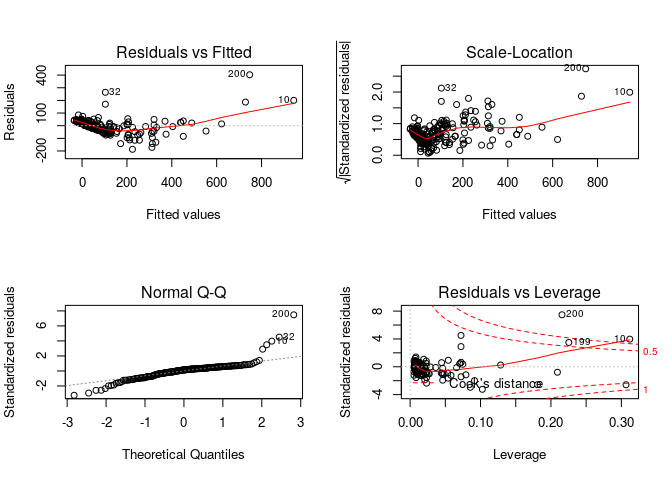
\includegraphics[width=0.7\linewidth]{SecAssignment_files/figure-html/unnamed-chunk-17-1.png}
	\caption{Residual Diagnostics as created by Base packages}
	\label{baseresplot}
\end{figure}


The generated residual plots are shown in figure \ref{baseresplot} and are fairly poorly generated, a better option would be
to use \verb|ggplot2|.


\hypertarget{ggplot2}{%
\subsubsection{ggplot2}\label{ggplot2}}

An implementation for \passthrough{\lstinline!ggplot2()!} to plot model
diagnostics has already been implemented\footnote{https://rpubs.com/therimalaya/43190}, and with some minor adjustment may be implemented here:

\begin{lstlisting}[language=R]
diagPlot<-function(model){
    p1<-ggplot(model, aes(.fitted, .resid))+geom_point(col = "IndianRed")
    p1<-p1+stat_smooth(method="loess", col = "Purple")+geom_hline(yintercept=0, col="red", linetype="dashed")
    p1<-p1+xlab("Fitted values")+ylab("Residuals")
    p1<-p1+ggtitle("Residual vs Fitted Plot")+theme_bw()
    
    p2<-ggplot(model, aes(qqnorm(.stdresid)[[1]], .stdresid))+geom_point(col = "IndianRed",na.rm = TRUE)
    p2<-p2+geom_abline(slope = 1, intercept = 0)+xlab("Theoretical Quantiles")+ylab("Standardized Residuals")
    p2<-p2+ggtitle("Normal Q-Q")+theme_bw()
    
    p3<-ggplot(model, aes(.fitted, sqrt(abs(.stdresid))))+geom_point(col = "IndianRed",na.rm=TRUE)
    p3<-p3+stat_smooth(method="loess",col = "Purple" , na.rm = TRUE)+xlab("Fitted Value")
    p3<-p3+ylab(expression(sqrt("|Standardized residuals|")))
    p3<-p3+ggtitle("Scale-Location")+theme_bw()
    
    p4<-ggplot(model, aes(seq_along(.cooksd), .cooksd))+geom_bar(stat="identity", position="identity")
    p4<-p4+xlab("Obs. Number")+ylab("Cook's distance")
    p4<-p4+ggtitle("Cook's distance")+theme_bw()
    
    p5<-ggplot(model, aes(.hat, .stdresid))+geom_point(col = "IndianRed", aes(size=.cooksd), na.rm=TRUE)
    p5<-p5+stat_smooth(method="loess",col = "Purple" , na.rm=TRUE)
    p5<-p5+xlab("Leverage")+ylab("Standardized Residuals")
    p5<-p5+ggtitle("Residual vs Leverage Plot")
    p5<-p5+scale_size_continuous("Cook's Distance", range=c(1,5))
    p5<-p5+theme_bw()+theme(legend.position="bottom")
    
    p6<-ggplot(model, aes(.hat, .cooksd))+geom_point(col = "IndianRed", na.rm=TRUE)+stat_smooth(method="loess",col = "Purple" , na.rm=TRUE)
    p6<-p6+xlab("Leverage hii")+ylab("Cook's Distance")
    p6<-p6+ggtitle("Cook's dist vs Leverage hii/(1-hii)")
    p6<-p6+geom_abline(slope=1, intercept = 0, color="gray", linetype="dashed")
    p6<-p6+theme_bw()
    
    return(list(rvfPlot=p1, qqPlot=p2, sclLocPlot=p3, cdPlot=p4, rvlevPlot=p5, cvlPlot=p6))
}
\end{lstlisting}

\begin{lstlisting}[language=R]
diagArray <- function(model){
grid.arrange(
diagPlot(model)$rvfPlot,
diagPlot(model)$qqPlot,
diagPlot(model)$rvlevPlot,
diagPlot(model)$cvlPlot)
}

diagArray(best.Mod.mlm)
\end{lstlisting}

\begin{figure}
	\centering
	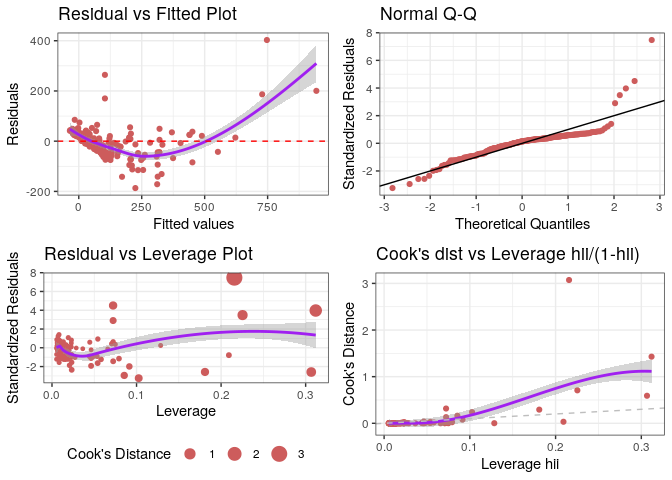
\includegraphics[width=0.7\linewidth]{SecAssignment_files/figure-html/unnamed-chunk-19-1.png}
	\caption{Residual Plots for the Multiple Linear Regression Model}
	\label{MultLinResP}
\end{figure}

\newpage

The residual plot created by \verb|ggplot2| are shown in figure \ref{MultLinResP} and appear somewhat non-Gaussian in the plot of the fitted
values against the model residuals, there appears to be a concave up
pattern in the residuals across the fitted values, the normal QQ plot
appears to deviate significantly from the line and there appears to be
values with high points of leverage.

It appears that the assumption of normally distributed residuals may be
violated.

\hypertarget{transform-the-data-to-overcome-diagnostic-issues.}{%
\subsection{(5) Transform the Data to Overcome Diagnostic
issues.}\label{transform-the-data-to-overcome-diagnostic-issues.}}

An appropriate transform for the data in order to address the
non-normality of the residuals would be a concave transform of the
response.

\begin{lstlisting}[language=R]
cpu$rootPerformance <- sqrt(cpu$Performance)

hist <- ggplot(cpu, aes(x = Performance)) +
  geom_histogram(binwidth = 80) +
  theme_classic() +
  labs(y = "Observations", title = "Histogram of Performance")

loghist <- ggplot(cpu, aes(x = rootPerformance)) +
  geom_histogram(binwidth = 1) +
  theme_classic() +
  labs(y = "Observations", title = "Histogram of Performance", x = "Root-Performance")


ggarrange(hist, loghist, ncol = 2)
\end{lstlisting}

\begin{figure}
	\centering
	
\includegraphics[width=0.7\linewidth]{SecAssignment_files/figure-html/unnamed-chunk-20-1.png}
	\caption{Histogram of Performance Variable}
	\label{histPerf}
\end{figure}


The preceding code generated the histograms shown in figure \ref{histPerf} which clearly demonstrates skew-right, potentially log-normal response data, hence a
$\log$-transform may be appropriate, however a $\log$-transform, when applied significantly
compromised the normality of the residuals across the fitted data, and
hence a root-transform is used instead, the residuals of the root transform are shown in figure \ref{rootresD}:

\begin{lstlisting}[language=R]
best.Mod.mlm <- lm(rootPerformance ~ MinimumMainMemory + MaximumMainMemory + CacheSize + MaximumNumberOfChannels, cpu)

diagArray(best.Mod.mlm)
\end{lstlisting}

\begin{figure} [h]
	\centering
	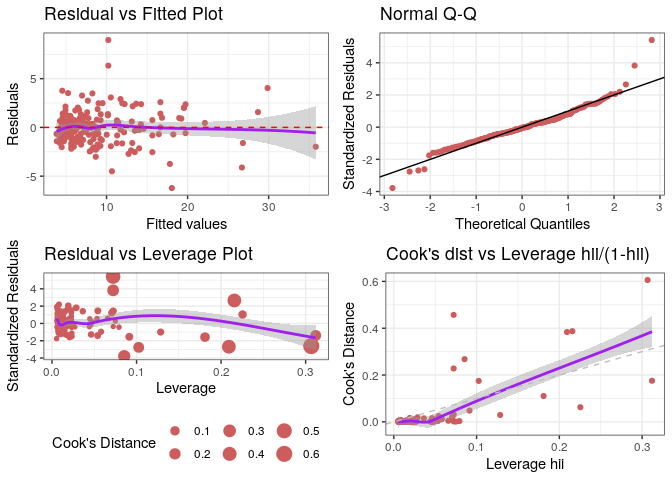
\includegraphics[width=0.7\linewidth]{SecAssignment_files/figure-html/unnamed-chunk-21-1.png}
	\caption{Residuals Diagnostics of Root Transformed Response predicted by a multiple linear regression}
	\label{rootresD}
\end{figure}




The residuals hence generated are shown in figure \ref{rootresD}, following the transform, they are sufficiently normal in order
to accept the model; although the model does appear to have a few points of
high leverage.

The optimal multiple linear regression model is hence:

{ \small
\begin{align}
Y_{\textsf{Perf}} = \left( 3.7 + 0.000363 \times \textsf{MinMem}  + 0.000221 \times \textsf{MaxMem} + 0.03723 \times \textsf{Cache} + 0.0248 \times \textsf{MaxChannels} \right)^2 \label{bestMultTrans}
\end{align}
}

\newpage

\hypertarget{question-2}{%
\section{Question 2}\label{question-2}}

\hypertarget{choose-an-appropriate-polynomial-attribute}{%
\subsection{(1) Choose an appropriate polynomial
attribute}\label{choose-an-appropriate-polynomial-attribute}}

Select the most suitable attribute of CPU that can be used to predict
accurately the performance of CPU using Polynomial Regression.

\hypertarget{consider-cycle-time}{%
\subsubsection{Consider Cycle Time}\label{consider-cycle-time}}

The plot at figure \ref{sp-1} shows a very strong non-linear, possibly
directly inversely proprtional, relationship between CycleTime and
performance, by the nature of the strong visual relationship between cycle time and
performance, it will be considered as a potential attribute to predict
CPU performance using a polynomial model.

Create the various models:

\begin{lstlisting}[language=R]
set.seed(2)
maxdeg <- 15

modsCT <- vector(mode = "list", length = maxdeg)
modsCT[[1]] <- glm(Performance ~ I(1/CycleTime), data = cpu)
names(modsCT)[1] <- "Hyperbolic"

for(i in 1:maxdeg){
modsCT[[i+1]] <-  glm(Performance ~ poly(CycleTime, i, raw = TRUE), data = cpu)
names(modsCT)[i+1] <- paste("Degree ", i)
}
\end{lstlisting}

Perform cross-Validation across the models

\begin{lstlisting}[language=R]
CycTime_CrossValDF <- tibble("Model" = factor(names(modsCT), levels = names(modsCT), ordered = TRUE), "CVError" = rep(NA, maxdeg+1))


CycTime_CrossValDF[(1), "CVError"] <- sqrt(cv.glm(data = cpu, glmfit = modsCT[[1]], K = 10)$delta[1])
for (i in 1:(maxdeg)) {
  CycTime_CrossValDF[(i+1), "CVError"] <- sqrt(cv.glm(data = cpu, glmfit = modsCT[[(i+1)]], K = 10)$delta[1])
}
\end{lstlisting}

Now plot the CV Error

\begin{lstlisting}[language=R]
ggplot(data = CycTime_CrossValDF, aes(x = factor(Model, ordered = TRUE), y = CVError, group = 1)) +
  geom_point(col = "IndianRed", size = 5) +
geom_line(col = "Purple") +
  theme_classic() + 
  labs(x = "Polynomial Model", y = "Expected Testing Error", title = "Cross-Validation for Cycle Time") +
  geom_vline(xintercept =  1, col = "RoyalBlue") +
  geom_vline(xintercept = which.min(CycTime_CrossValDF[[ "CVError"]]), col = "brown") +
  theme(axis.text.x = element_text(angle = 90, hjust = 1))
\end{lstlisting}

\begin{figure}
	\centering
	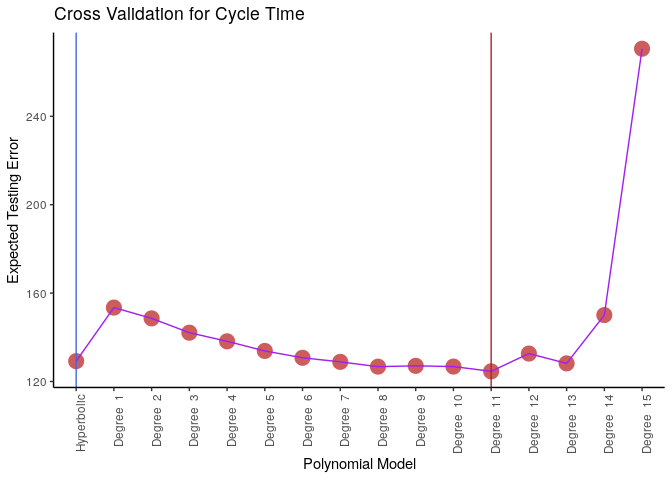
\includegraphics[width=0.7\linewidth]{SecAssignment_files/figure-html/unnamed-chunk-24-1.png}
	\caption{Plot of cross-validation for given polynomial model, The best performing model is either a hyperbola or an 11th degree polynomial}
	\label{cvpoly}
\end{figure}


\newpage


The plot of Error and Polynomial degree is shown in figure \ref{cvpoly}, although the Cycle Time performs well as a predictive feature within a
polynomial model of a high degree, the simplest model that performs
equaly as well is the hyperbolic model. The simpler model should be
accepted because the higher degree polynomial will increase the
variance of the model without significantly improving the performance of
the model. When Cycle time is chosen as the best attribute to model the
performance of the CPU, the hyperbolic model is the optimal model:

\begin{align}
Y_{Perf} = \frac{8229.468}{X_{CycTime}} \label{hypcyc}
\end{align}


\hypertarget{choose-the-best-performing-variable}{%
\subsubsection{Choose the Best Performing
variable}\label{choose-the-best-performing-variable}}

However it may be such that cycle time is not the most appropriate
variable, moreover a hyperbola is not a polynomial curve but a \textit{rational} curve.

 In order to determine the best single attribute that may be
used to predict performance by way of a polynomial model the \emph{best
attributes} algorithm may be extended:

\begin{enumerate}
\def\labelenumi{\arabic{enumi}.}
\tightlist
\item
  For all predictors:

\begin{itemize}
\tightlist
\item
  Fit all hyperbolic, linear and 2nd to nth degree polynomial models
  using only a sinle predictor, choose the predictor that returns the
  lowest training error
\item
  Repeat for all Predictors
\end{itemize}


\def\labelenumi{\arabic{enumi}.}
\setcounter{enumi}{1}
\tightlist
\item
  Select a single bestmodel from among the hyperbolic, linear and
  polynomial models by using cross-validation.
\end{enumerate}

This resulting model will be the best performing model given the
constraints that it must be a polynomial model with only a single
attribute.

\hypertarget{implement-the-algorithm}{%
\paragraph{Implement the Algorithm}\label{implement-the-algorithm}}

Set the seed, create a tibble and create a data frame in which to store
the best predictors:

\begin{lstlisting}[language=R]
# Questoin 2 Scratch ------------------------------------------------------
set.seed(31415)


mdg <- 9 # Maximum Degree to Consider in Question 2

cpu <- as_tibble(cpu)
predictors <- select(cpu, c( "CycleTime", "MinimumMainMemory", "MaximumMainMemory", "CacheSize", "MinimumNumberOfChannels", "MaximumNumberOfChannels"))
names(cpu)
\end{lstlisting}

\begin{lstlisting}
## [1] "CycleTime"               "MinimumMainMemory"      
## [3] "MaximumMainMemory"       "CacheSize"              
## [5] "MinimumNumberOfChannels" "MaximumNumberOfChannels"
## [7] "Performance"             "Frequency"              
## [9] "rootPerformance"
\end{lstlisting}

\begin{lstlisting}[language=R]
BestPred <- data.frame("Degree" = 1:(mdg+1), "BestAttribute" = rep(NA, (mdg+1)))
\end{lstlisting}

Now create a loop to determine the best attribute for each corresponding
model:

\begin{lstlisting}[language=R]
# Lin to 6th deg


BestPred <- data.frame("Degree" = 1:(mdg+1), "BestAttribute" = rep(NA, (mdg+1)))

for (j in (1:mdg)) {
  
RSSVals <- data.frame(names(predictors), "RSS" = 1:length(predictors))
  for (i in 1:length(predictors)) {
    
    RSSVals[i,2] <- (glm(cpu$Performance ~ poly(as_vector(predictors[i]), j))$residuals)^2 %>% sum()
    
  }

BestPred[j,2] <-  as.character(RSSVals[which.min(RSSVals[,2]),1][1])
}

# Hyperbolic

RSSVals <- data.frame(names(predictors), "RSS" = 1:length(predictors))
for (i in 1:length(predictors)) {
  
  RSSVals[i,2] <- (glm(cpu$Performance ~ (1/as_vector(predictors[i])))$residuals)^2 %>% sum()
  
}

BestPred$Degree[(mdg+1)] <- -1
BestPred[(mdg+1),2] <-  as.character(RSSVals[which.min(RSSVals[,2]),1][1])

BestPred
\end{lstlisting}

\begin{lstlisting}
##    Degree     BestAttribute
## 1       1 MaximumMainMemory
## 2       2 MaximumMainMemory
## 3       3 MaximumMainMemory
## 4       4 MaximumMainMemory
## 5       5 MaximumMainMemory
## 6       6 MaximumMainMemory
## 7       7 MaximumMainMemory
## 8       8 MaximumMainMemory
## 9       9 MaximumMainMemory
## 10     -1         CycleTime
\end{lstlisting}

\hypertarget{use-10-fold-cv-to-select-the-optimal-model}{%
\subsection{(2) Use 10-fold CV to Select the Optimal
Model}\label{use-10-fold-cv-to-select-the-optimal-model}}

Now that we have the best attribute for any given model, we may use
cross-validation in order to decide upon the best model, first however
create a list of models and a data frame in which to store the CV
errors:

\begin{lstlisting}[language=R]
# Now I have to perform cross-validation on every model
## Create a list of models

### Create the model names
modnames <- rep(NA, (mdg+1))
for (i in (1:(mdg+1))) {
 modnames[i] <- paste("Degree ", i) 
  
}
modnames[mdg+1] <- "Hyperbolic"

### Create the list of Models
mods <- vector(mode = "list", length = length(modnames))
names(mods) <- modnames

### Assign the models

for (i in 1:mdg) {
 mods[[i]] <-  glm(formula = paste("Performance ~ ", BestPred[i,2]), data = cpu)
}

mods[[(mdg+1)]] <- glm(Performance ~ I(1/CycleTime), data = cpu)


## Use the list to perform Cross Validation

### Make a data frame to track the expected error
BestPred$CVError <- rep(NA, nrow(BestPred))
\end{lstlisting}

Now actually perform the 10-fold cross-validation:

\begin{lstlisting}[language=R]
### Compute the CV Error
for (r in 1:nrow(BestPred)) {
BestPred[r,3] <- sqrt(cv.glm(data = cpu, glmfit = mods[[r]], K = 10)$delta[1])
}
\end{lstlisting}

\newpage

Now clean up the names and plot the cross-validation:

\begin{lstlisting}[language=R]
BestPred$names <- names(mods)
BestPred <- arrange(.data = BestPred, sort.by = Degree)
names(BestPred)[2] <- "Best Attribute"


ggplot(BestPred, aes(x = factor(Degree, labels = BestPred$names, ordered = TRUE), y = CVError, group = 1)) + 
  geom_point(aes(shape = `Best Attribute`, col = `Best Attribute`),  size = 5) +
  geom_line() +
  theme_classic()  +
  labs(x = "Model Type",
       y = TeX("Estimated Testing Error $\\pm $ Performance"),
       title = "Cross Validation of Different Models") +
  geom_vline(xintercept = which.min(BestPred$CVError))+
  theme(axis.text.x = element_text(angle = 90, hjust = 1))
\end{lstlisting}



\begin{figure}
	\centering
	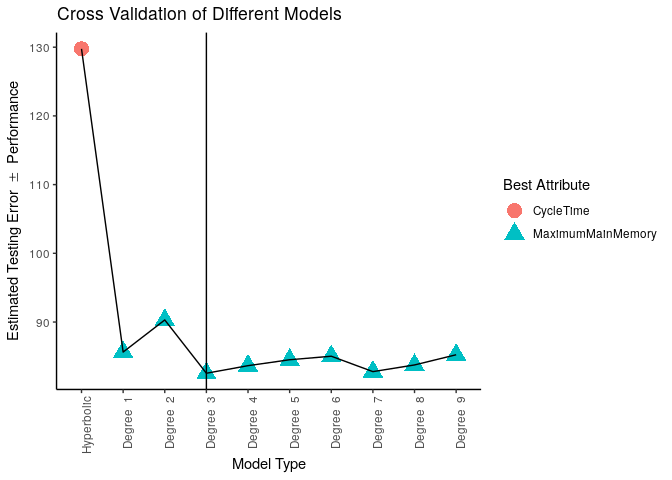
\includegraphics[width=0.7\linewidth]{SecAssignment_files/figure-html/unnamed-chunk-29-1.png}
	\caption{A plot of the Expected testing error, as predicted by 10-fold CV given the specific model type, the model corresponds to the single best performing attribute for that model.}
	\label{cfPolyBest}
\end{figure}


\newpage


The algorithm produces the plot shown in figure \ref{cfPolyBest} and shows that the best model will be a cubic model using the maximum memory attribute, if leave-one out CV is performed instead the optimal model will be found to be the same, hence the best polynomial model, using only
one attribute, is a 3rd degree polynomial using
\passthrough{\lstinline!MaximumMainMemory!}:

\begin{lstlisting}[language=R]
bestPoly <- lm(Performance ~ poly(MaximumMainMemory, 3), cpu)
summary(bestPoly)
\end{lstlisting}

\begin{lstlisting}
## 
## Call:
## lm(formula = Performance ~ poly(MaximumMainMemory, 3), data = cpu)
## 
## Residuals:
##     Min      1Q  Median      3Q     Max 
## -325.93  -22.30   -9.03   10.59  333.19 
## 
## Coefficients:
##                             Estimate Std. Error t value Pr(>|t|)    
## (Intercept)                  105.617      4.579  23.067   <2e-16 ***
## poly(MaximumMainMemory, 3)1 2001.742     66.194  30.240   <2e-16 ***
## poly(MaximumMainMemory, 3)2  684.557     66.194  10.342   <2e-16 ***
## poly(MaximumMainMemory, 3)3  -79.978     66.194  -1.208    0.228    
## ---
## Signif. codes:  0 '***' 0.001 '**' 0.01 '*' 0.05 '.' 0.1 ' ' 1
## 
## Residual standard error: 66.19 on 205 degrees of freedom
## Multiple R-squared:  0.833,  Adjusted R-squared:  0.8306 
## F-statistic:   341 on 3 and 205 DF,  p-value: < 2.2e-16
\end{lstlisting}

so the model optimal polynomial model is:

\begin{align}
Y_{Perf} = 106 + 2002 \times \textsf{Mem} + 685 \times \textsf{Mem}^2 -80 \times \textsf{Mem}^3 \label{bestpoly}
\end{align}


\hypertarget{comment-on-the-accuracy-of-the-model}{%
\subsection{(3) Comment on the Accuracy of the
Model}\label{comment-on-the-accuracy-of-the-model}}

The expected RMSE of the model on unseen data is approximately 82.5 as
determined by 10-fold cross-validation, so it would be expected that
this model will make predictions with an expected error of 82.5, this is
significantly less than the standard deviation of the CPU performance
and so the model would be expected to perform significantly better than
mere chance.

\hypertarget{model-diagnostics}{%
\subsection{(4) Model Diagnostics}\label{model-diagnostics}}

The residuals of the best performing model may be considered using the previously defined function and are shown in figure \ref{polyresd}:

\begin{lstlisting}[language=R]
diagArray(bestPoly)
\end{lstlisting}


\begin{figure}
	\centering
	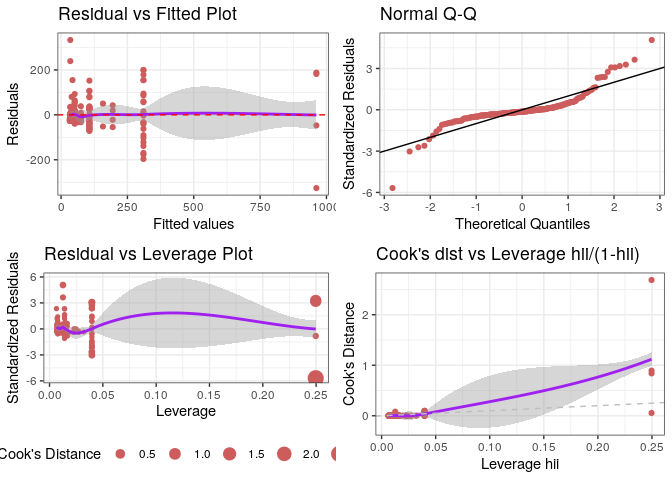
\includegraphics[width=0.7\linewidth]{SecAssignment_files/figure-html/unnamed-chunk-31-1.png}
	\caption{Residual Diagnostics corresponding to the fitted model in equation \eqref{bestpoly}}
	\label{polyresd}
\end{figure}




The residuals appear to be bunched up to the left, however, there is no
distinct pattern; although the residuals do not necessarily resemble normally
distributed data, owing to the lack of centred observations, there is insufficient evidence to contradict the assumption of non-normality. 

The normal Q-Q plot has a wave to it and so the
distribution of the residuals would hence correspond to a `fat-tailed'
distribution.

The residual plots are not sufficiently non-normal to reject the model
on grounds of non-normal residuals. Hence the attribute
\passthrough{\lstinline!MaximumMainMemory!} is accepted as the most
suitable attribute for the most optimal single variable polynomial
regression, as measured by 10-fold cross-validation and the model in \eqref{bestpoly} is accepted.

\newpage

\hypertarget{question-3---wine-trees}{%
\section{Question 3}\label{question-3---wine-trees}}

\hypertarget{create-a-test-and-training-set}{%
\subsection{(1) Create a Test and Training
set}\label{create-a-test-and-training-set}}

Divide the dataset into Training set with 4000 observations and assign the
rest of the observations into a test set. 

The data set may be imported and a training set indexed thusly:

\begin{lstlisting}[language=R]
set.seed(10)

#Import the data
wine <- as_tibble(read.csv(file = "./Code/Datasets/Wine.csv", header = TRUE, sep = ","))
glimpse(wine)
\end{lstlisting}

\begin{lstlisting}[basicstyle=\footnotesize \ttfamily]
## Observations: 4,898
## Variables: 12
## $ WineQuality        <int> 6, 6, 6, 6, 6, 6, 6, 6, 6, 6, 5, 5, 5, 7, 5, ...
## $ FixedAcidity       <dbl> 7.0, 6.3, 8.1, 7.2, 7.2, 8.1, 6.2, 7.0, 6.3, ...
## $ VolatileAcidity    <dbl> 0.27, 0.30, 0.28, 0.23, 0.23, 0.28, 0.32, 0.2...
## $ CitricAcid         <dbl> 0.36, 0.34, 0.40, 0.32, 0.32, 0.40, 0.16, 0.3...
## $ ResidualSugar      <dbl> 20.70, 1.60, 6.90, 8.50, 8.50, 6.90, 7.00, 20...
## $ Chlorides          <dbl> 0.045, 0.049, 0.050, 0.058, 0.058, 0.050, 0.0...
## $ FreeSulfurDioxide  <dbl> 45, 14, 30, 47, 47, 30, 30, 45, 14, 28, 11, 1...
## $ TotalSulfurDioxide <dbl> 170, 132, 97, 186, 186, 97, 136, 170, 132, 12...
## $ Density            <dbl> 1.0010, 0.9940, 0.9951, 0.9956, 0.9956, 0.995...
## $ PH                 <dbl> 3.00, 3.30, 3.26, 3.19, 3.19, 3.26, 3.18, 3.0...
## $ Sulphates          <dbl> 0.45, 0.49, 0.44, 0.40, 0.40, 0.44, 0.47, 0.4...
## $ Alcohol            <dbl> 8.8, 9.5, 10.1, 9.9, 9.9, 10.1, 9.6, 8.8, 9.5...
\end{lstlisting}

\begin{lstlisting}[language=R]
# Create a training set
train <- sample(1:(nrow(wine)), size = 4000)
wine.test   <- slice(wine, -train)
wine.train <- slice(wine, train)
\end{lstlisting}

\hypertarget{build-a-decision-tree}{%
\subsection{(2) Build a Decision Tree}\label{build-a-decision-tree}}

A decision tree may be constructed by using the following code:

\begin{lstlisting}[language=R]
wine.tree <- tree(WineQuality ~ ., wine.train)
summary(wine.tree)
paste("SD of Quality: ", sd(wine$WineQuality))
paste("Average Wine Quality: ", mean(wine$WineQuality))
\end{lstlisting}

\begin{lstlisting}
## 
## Regression tree:
## tree(formula = WineQuality ~ ., data = wine.train)
## Variables actually used in tree construction:
## [1] "Alcohol"           "VolatileAcidity"   "FreeSulfurDioxide"
## Number of terminal nodes:  5 
## Residual mean deviance:  0.5788 = 2312 / 3995 
## Distribution of residuals:
##    Min. 1st Qu.  Median    Mean 3rd Qu.    Max. 
## -3.5890 -0.3856  0.1013  0.0000  0.6144  3.6140

## [1] "SD of Quality:  0.885638574967831"
## [1] "Average Wine Quality:  5.87790935075541"
\end{lstlisting}



reducing the number of terminal nodes (known as `pruning' the tree) may
elicit better performance from the model, this ideal number of terminal
nodes may be considered by using cross-validation:

\begin{lstlisting}[language=R]
wine.treeCV <- cv.tree(wine.tree)

WineCVError <- tibble("Nodes" = wine.treeCV$size, "RSS" = wine.treeCV$dev, "MSE" = (wine.treeCV$dev)/length(train), "RMSE" = sqrt((wine.treeCV$dev)/length(train)))

ggplot(WineCVError, aes(x = Nodes, y = RMSE, group = 1)) +
  geom_point(col = "#B223F5", size = 5) +
  geom_line(col = "#DBA0D6") +
  theme_classic2() +
  labs(title = "Cross-Validation Error", y = TeX("Expected Error $ \\left(E ( \\epsilon) \\right)$"), caption = "RMSE is an estimation of the mean residual value, hence it is expressed that RMSE is the expected model error") +
  geom_vline(xintercept = as.integer(summary(wine.treeCV)[1,1]), col = c("#AB0FFF")) +
  geom_hline(yintercept = min(WineCVError$RMSE), col = c("#AB0FFF")) +
  annotate(geom = "text", y = (min(WineCVError$RMSE)+sd(WineCVError$RMSE)), x = (4), label = paste("Expected Error: ", signif(min(WineCVError$RMSE), 3))) 
\end{lstlisting}



\begin{figure}
	\centering
	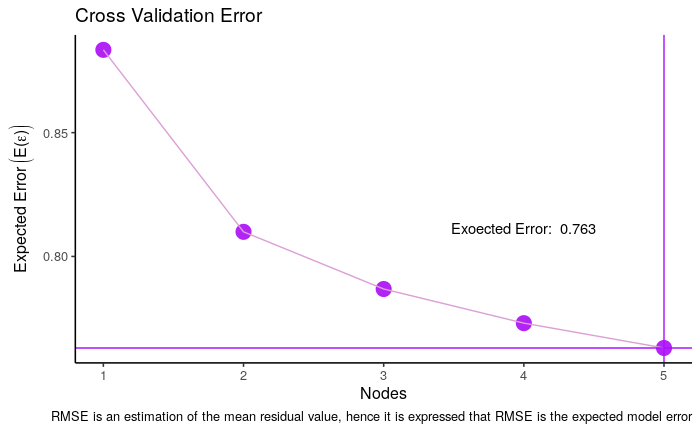
\includegraphics[width=0.7\linewidth]{SecAssignment_files/figure-html/unnamed-chunk-34-1.png}
	\caption{Expected testing error }
	\label{cvtree}
\end{figure}




The preceding code produces the plot in figure \ref{cvtree} which suggests that the model initially used, with 5 nodes, is the best
performing model, hence a 5-node tree model is accepted and depicted in figure \ref{basetreemodreg}:

\begin{lstlisting}[language=R]
plot(wine.tree)
text(wine.tree, pretty = 1, cex = 0.75)
\end{lstlisting}

\begin{figure}
	\centering
	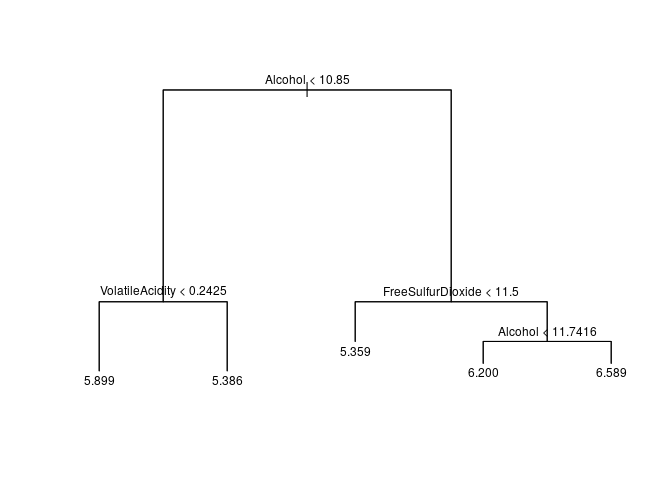
\includegraphics[width=0.7\linewidth]{SecAssignment_files/figure-html/unnamed-chunk-35-1.png}
	\caption{Regression Tree Model of Wine Quality}
	\label{basetreemodreg}
\end{figure}




\hypertarget{superior-plot}{%
\subsubsection{Superior Plot}\label{superior-plot}}

A superior plot (and automatic cross-validation) may be produced by
using the \passthrough{\lstinline!rpart()!} function:

\begin{lstlisting}[language=R]
WineModTree.rpart <- rpart(formula = WineQuality~ ., data = wine.train)
WineModTree.plot  <- rpart.plot(WineModTree.rpart, box.palette="OrGy", shadow.col="gray", nn=TRUE)
\end{lstlisting}

\begin{figure}
\centering
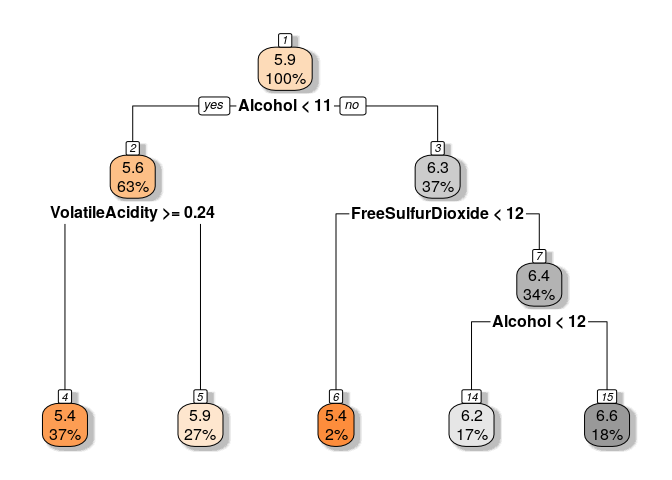
\includegraphics[width=0.7\linewidth]{SecAssignment_files/figure-html/tree-1.png}
\caption{Tree Model for Wine Quality}
\label{rpartregtree}
\end{figure}

which produces the plot shown in \ref{rpartregtree}


\hypertarget{significant-attributes}{%
\subsubsection{Significant Attributes}\label{significant-attributes}}

It can be oveserved from figure \ref{rpartregtree} that in creating this model
only the measurements of alcohol, volatile acidity and free $\textsf{SO}_2$ are found to be significant, the mean square error (MSE) of this
model (errounesly listed as deviance by this package) is 0.58, which is
a reasonably low training error, given that this is significantly lower
than the standard deviation of the wine quality which is 0.89 with an
average wine quality value of 5.9.

\newpage

\hypertarget{model-performance}{%
\subsection{(3) Model Performance}\label{model-performance}}

\hypertarget{comparison-to-testing-data}{%
\paragraph{Comparison to testing
data}\label{comparison-to-testing-data}}

\begin{lstlisting}[language=R]
wineTreePreds.test <- predict(object = wine.tree, newdata = wine.test)

rmse <- function(pred, obs){
  if(require("tidyverse")){
    (pred-obs)^2 %>% mean %>% sqrt()
  } else{
    print("Install Tidyverse first")
  }
}

wineTree.rmse <- rmse(pred = wineTreePreds.test, obs = wine.test$WineQuality)
\end{lstlisting}

\hypertarget{comment-on-the-error}{%
\subsubsection{Comment on the Error}\label{comment-on-the-error}}

Cross validation provides that the expected error by using this model is
0.77 units of quality, the same expected error value is returned from
fitting the model to testing data, the standard deviation (i.e.~the
expected difference between values of wine quality) is about 0.89, so
this model is expected, by cross-validation, to perform better than mere
chance.

\hypertarget{build-a-categorical-decision-tree}{%
\subsection{(4) Build a Categorical Decision
tree}\label{build-a-categorical-decision-tree}}

First create a factor of variables for high and low wine quality

\begin{lstlisting}[language=R]
wine$WineCat <- ifelse(wine$WineQuality > 6, "high", "low")
wine$WineCat <- factor(x = wine$WineCat, levels = c("low", "high"), ordered = TRUE, nmax = 2)

wine.test  <- slice(wine, -train)
wine.train <- slice(wine, train)
\end{lstlisting}

the tree model may be constructed thusly:

\begin{lstlisting}[language=R]
wineCat.tree <- tree(WineCat ~ . -WineQuality, wine.train)
# plot(wineCat.tree)
# text(wineCat.tree, pretty = 1, cex = 0.75)
\end{lstlisting}

A better performing model may be found by `pruning' the tree, specifying the \verb|FUN| parameter will cause the cross-validation algorithm to show
preference for a model that reduces the misclassification rate (as opposed to cost complexity pruning), the corresponding plot of Cross-Validation errors is shown in figure \ref{cvtreeclass} and is generated by the following code:

\begin{lstlisting}[language=R]
wineCat.treeCV <- cv.tree(object = wineCat.tree, FUN = prune.misclass, K = 10)

wineCat.treeCV
\end{lstlisting}

\begin{lstlisting}
## $size
## [1] 6 5 3 1
## 
## $dev
## [1] 835 835 837 857
## 
## $k
## [1] -Inf  0.0  3.5 10.5
## 
## $method
## [1] "misclass"
## 
## attr(,"class")
## [1] "prune"         "tree.sequence"
\end{lstlisting}

\begin{lstlisting}[language=R]
summary(wineCat.tree)
\end{lstlisting}

\begin{lstlisting}
## 
## Classification tree:
## tree(formula = WineCat ~ . - WineQuality, data = wine.train)
## Variables actually used in tree construction:
## [1] "Alcohol"         "VolatileAcidity"
## Number of terminal nodes:  6 
## Residual mean deviance:  0.8307 = 3318 / 3994 
## Misclassification error rate: 0.2065 = 826 / 4000
\end{lstlisting}

\begin{lstlisting}[language=R]
WineCatCVError <- tibble("Nodes" = as.numeric(wineCat.treeCV$size), "MisClas" = wineCat.treeCV$dev/length(train))
WineCatCVError <- arrange(WineCatCVError, Nodes)

WineCatCVError <- tibble("Nodes" = factor(x = WineCatCVError[[ "Nodes"]], levels = WineCatCVError[[ "Nodes"]], ordered = TRUE), "MisClas" = WineCatCVError[[ "MisClas"]])
bestNode <- WineCatCVError[[ "Nodes"]][which.min(WineCatCVError[["MisClas"]])]
bestMisclas <- WineCatCVError[[ "MisClas"]][bestNode]

ggplot(WineCatCVError, aes(x = Nodes, y = MisClas, group = 1)) +
  geom_point(col = "#B223F5", size = 5) +
  geom_line(col = "#DBA0D6") +
  theme_classic2() +
  labs(title = "Cross Validation Error", y = "Misclassificatoin Rate", caption = "Misclassification Rate is a measurement of the expected frequency of misclassification as determined by Cross Validation") +
  geom_vline(xintercept = as.integer(bestNode), col = c("#AB0FFF")) +
  geom_hline(yintercept = bestMisclas, col = c("#AB0FFF")) +
  annotate(geom = "text", y = bestMisclas+sd(WineCatCVError$MisClas), x = (1.1+3), label = paste("Misclassification Rate: \n", signif(min(WineCatCVError$MisClas), 3))) 
\end{lstlisting}

\begin{figure}[h]
	\centering
	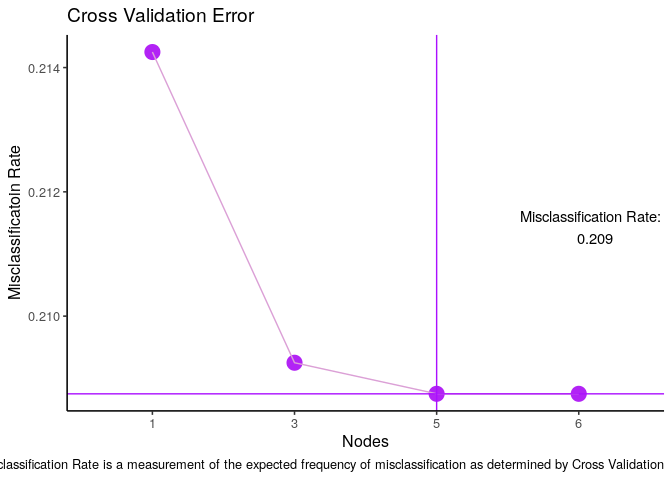
\includegraphics[width=0.7\linewidth]{SecAssignment_files/figure-html/unnamed-chunk-40-1.png}
	\caption{A plot of the expected testing error, as determined by 10-fold cross validation, corresponding to the number of final nodes for a categorical tree model of wine quality}
	\label{cvtreeclass}
\end{figure}


The expected misclassification rate on unseen data for this model, as
predicted by cross-validation, will be minimised by choosing five nodes and hence the model will be pruned from six to five terminal nodes, this
can be acheived by using the \passthrough{\lstinline!prune.misclass()!}
function and is depicted in figure \ref{treecatwine}:

\begin{lstlisting}[language=R]
wineCat.tree.prune <- prune.misclass(wineCat.tree, best = bestNode)
plot(wineCat.tree.prune)
text(wineCat.tree.prune, pretty = 1, cex = 0.75)
\end{lstlisting}

\begin{figure}[h!]
	\centering
	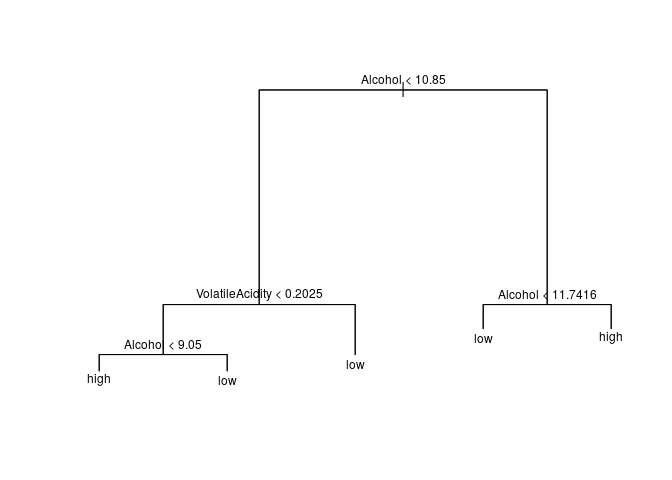
\includegraphics[width=0.7\linewidth]{SecAssignment_files/figure-html/unnamed-chunk-41-1.png}
	\caption{Model of High/Low Wine Quality, the number of 'leaves' on this tree model has been selected in order to minimise the testing error of the model as determined by cross-validation}
	\label{treecatwine}
\end{figure}

\newpage

\hypertarget{comment-on-the-performance-of-the-model}{%
\subparagraph{(5) Comment on the performance of the
model}\label{comment-on-the-performance-of-the-model}}

the model can be applied to the testing data in order to assess the rate of
misclassification:

\begin{lstlisting}[language=R]
WineTreeCatPreds <- predict(object = wineCat.tree.prune, newdata = wine.test, type = "class")
WineTestObs <- wine.test$WineCat


# Now create the confusion Matrix
  # This package prevents making mistakes
  conf.mat <-   caret::confusionMatrix(data = WineTreeCatPreds, reference = WineTestObs)
  conf.mat
\end{lstlisting}

\begin{lstlisting}
## Confusion Matrix and Statistics
## 
##           Reference
## Prediction low high
##       low  591  107
##       high 101   99
##                                           
##                Accuracy : 0.7684          
##                  95% CI : (0.7394, 0.7956)
##     No Information Rate : 0.7706          
##     P-Value [Acc > NIR] : 0.5813          
##                                           
##                   Kappa : 0.3381          
##                                           
##  Mcnemar's Test P-Value : 0.7288          
##                                           
##             Sensitivity : 0.8540          
##             Specificity : 0.4806          
##          Pos Pred Value : 0.8467          
##          Neg Pred Value : 0.4950          
##              Prevalence : 0.7706          
##          Detection Rate : 0.6581          
##    Detection Prevalence : 0.7773          
##       Balanced Accuracy : 0.6673          
##                                           
##        'Positive' Class : low             
## 
\end{lstlisting}

\begin{lstlisting}[language=R]
   mis.mat <- table("prediction" = WineTreeCatPreds, "reference" = WineTestObs)
    mcr <- signif((mis.mat[1,2]+mis.mat[2,1])/sum(mis.mat),2)
    mcr
\end{lstlisting}

\begin{lstlisting}
## [1] 0.23
\end{lstlisting}

The misclassification error rate on the testing data is 23\%, this is
comparable with what was predicted via cross-validation which returned
20.65\%, this misclassification rate corresponds to a tree model trained
to minimise the cross-validation misclassification rate (as opposed to
cost complexity).

This misclassification rate is quite high, however for the trade off of
interpretability, this is still an acceptable model. It's very
interesting that a good wine is essenitally synonymous with a strong
wine.

\newpage

\hypertarget{question-4}{%
\section{Question 4}\label{question-4}}

\hypertarget{design-a-support-vector-machine}{%
\subsection{(1) Design a Support Vector
Machine}\label{design-a-support-vector-machine}}

\hypertarget{create-a-categorical-variable}{%
\subsubsection{Create a categorical
Variable}\label{create-a-categorical-variable}}

Classify CPU performance as an ordered factor with levels of
\passthrough{\lstinline!high!} and \passthrough{\lstinline!low!}:

\begin{lstlisting}[language=R]
cpu <- select(cpu, -rootPerformance, -Frequency)
cpu$Performance <- if_else(cpu$Performance > 500, "high", "low")
cpu$Performance <- factor(cpu$Performance, c("low", "high"), ordered = TRUE)
\end{lstlisting}



\hypertarget{create-the-svm}{%
\paragraph{Create the SVM}\label{create-the-svm}}


A support Vector Classifier can be constructed with a linear kernel by
using the \passthrough{\lstinline!svm!} function:

\begin{lstlisting}[language=R]
set.seed(3)
cpu.svm <- svm(Performance ~ ., data = cpu, kernel = "linear", cost = 10, scale = FALSE)
\end{lstlisting}

Cross-validation can used in order to determine the best cost value via
the \passthrough{\lstinline!e1071::tune()!} function, the cost is, to a
degree, a measure of model flexibility and so there will be an optimal
cost value, for non-linear kernel's differing $\gamma$ values may be
considered as well and hence they will be included in a function call. The SVM can be created and the optimal cost and $\gamma$ values considered like so:

\begin{lstlisting}[language=R]
makeSVM <- function(formula = Performance ~ ., data = cpu, kernel = "linear", plotQ = TRUE){
# cpu.svm <- svm(Performance ~ ., data = cpu, kernel = "linear", cost = 10, scale = FALSE)

tune.cpu <- tune(method = svm, train.x = formula, data = data, kernel = kernel, ranges = list(cost = seq(from = 0.0001, to = 10, length.out = 50)), gamma = c(0.5, 1, 2, 3, 4))
summary(tune.cpu)
CVErrors <- as_tibble(summary(tune.cpu)[[7]])
CVErrors$error <- (CVErrors$error)

bestcost <- CVErrors$cost[CVErrors$error<=min(CVErrors[[ "error"]])][1]

tuneplot <- ggplot(CVErrors, aes(x = cost, y = error)) +
  geom_point(col = "#B223F5", size = 1) +
  geom_line(col = "#DBA0D6") +
  theme_classic2() +
  labs(title = "Cross Validation estimation of Error given Cost Parameter", y = "Error", x = "Cost", caption = paste("The optimal cost parameter appears to occur at a cost value of", signif(bestcost, 2))) +
  geom_hline(yintercept = (as.numeric(summary(tune.cpu)[2])), col = c("#AB0FFF")) + 
  geom_vline(xintercept = bestcost, col = c("#AB0FFF"))



if (plotQ) {
 return(tuneplot) 
} else {
  return(c("ErrorRate" = (as.numeric(summary(tune.cpu)[2]))))
}


}

# Consider using `kernlab::ksvm()`

makeSVM()
\end{lstlisting}

\begin{figure}
	\centering
	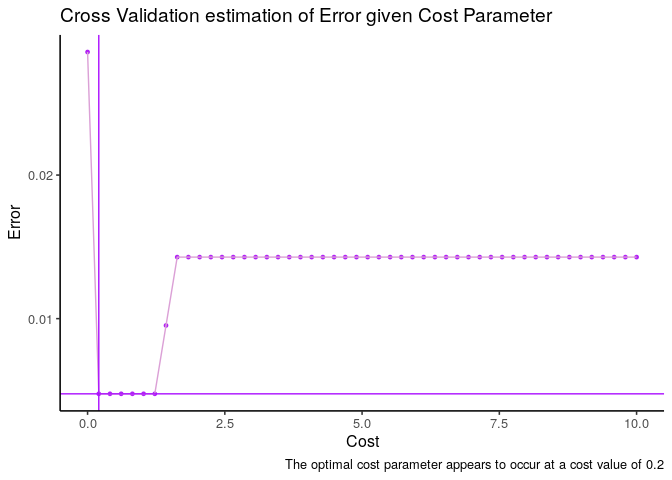
\includegraphics[width=0.7\linewidth]{SecAssignment_files/figure-html/unnamed-chunk-45-1.png}
	\caption{Expected testing error as determined by cross-validation given cost parameter of SVM}
	\label{linsvmcv}
\end{figure}


The results of 10-fold cross-validation are shown in figure \ref{linsvmcv}, it may be determined that the best cost value for
a linear kernel is 0.21.

\newpage

\hypertarget{compare-different-types-of-kernels}{%
\subsubsection{Compare Different Types of
Kernels}\label{compare-different-types-of-kernels}}

In order to compare the performance of the different type of SVM
kernel's a loop can be constructed and the expected testing error, as
determined by cross-validation, may be compared, this is depicted in figure \ref{svmcomp}:

\begin{lstlisting}[language=R]
models <- list("linear", "polynomial", "radial", "sigmoid")
KerDF <- tibble("Kernel" = c("Linear", "Polynomial", "Radial", "Sigmoid"), "CVError" = rep(NA, 4))


i <- 1
for (mod in models){
KerDF[i, 2] <- makeSVM(kernel = mod, plotQ = FALSE)
i <- i+1 
}

#KerDF

ggplot(KerDF, aes(x = Kernel, y = CVError, fill = Kernel)) +
  geom_col(alpha = 0.5) + 
  theme_bw() +
  labs(x = "Kernel Model", y = "Expected Misclassification Rate", title = "Cross Validated Errors for SVM Models")
\end{lstlisting}

\begin{figure}
	\centering
	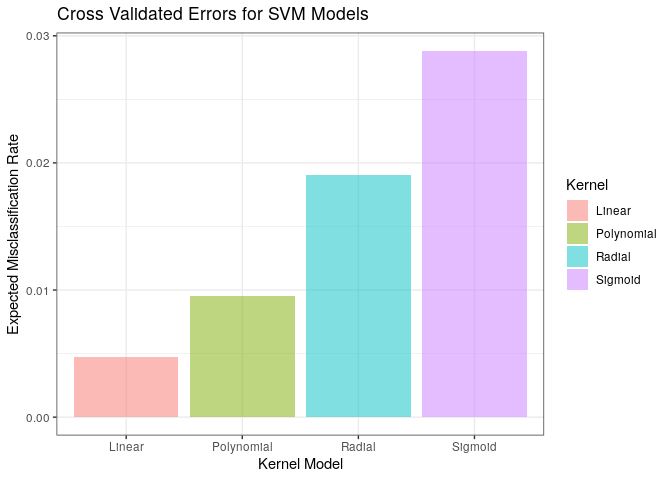
\includegraphics[width=0.7\linewidth]{SecAssignment_files/figure-html/unnamed-chunk-46-1.png}
	\caption{Comparison of expected testing error of best performing SVM models with differing kerne's, performance was determined by minimising expected testing error which was predicted using 10-fold cross-validation}
	\label{svmcomp}
\end{figure}

\newpage

The SVM using a linear kernel appears to have the lowest expected training error as
determined by 10-fold cross-validation, hence the linear SVM model is
accepted as the optimal SVM model with a cost parameter of 0.21:

\begin{lstlisting}[language=R]
cpu.svm <- svm(Performance ~ ., data = cpu, kernel = "linear", cost = 10, scale = FALSE)

tune.cpu <- tune(method = svm, train.x = Performance ~ ., data = cpu, kernel = "linear", ranges = list(cost = seq(from = 0.0001, to = 2, length.out = 30)))
#summary(tune.cpu)

summary(tune.cpu$best.model)
\end{lstlisting}

\begin{lstlisting}[basicstyle=\footnotesize \ttfamily]
## 
## Call:
## best.tune(method = svm, train.x = Performance ~ ., data = cpu, 
##     ranges = list(cost = seq(from = 1e-04, to = 2, length.out = 30)), 
##     kernel = "linear")
## 
## 
## Parameters:
##    SVM-Type:  C-classification 
##  SVM-Kernel:  linear 
##        cost:  0.2069862 
## 
## Number of Support Vectors:  7
## 
##  ( 3 4 )
## 
## 
## Number of Classes:  2 
## 
## Levels: 
##  low high
\end{lstlisting}


\hypertarget{The-Optimal-SVM}{%
	\paragraph{The Optimal SVM}\label{create-the-svm}}



The \passthrough{\lstinline!svm()!} function has the capacity to apply to more than
linear kernels, it is hence not simple to return the coefficients of a linear
decision boundary for higher dimensions and so this will be omitted. 

%\footnote{\href{https://www.datacamp.com/community/tutorials/support-vector-machines-r}{Data Camp SVM}}

\hypertarget{what-is-the-peformance}{%
\subsection{(2) What is the Performance?}\label{what-is-the-peformance}}

The error measurement returned by the \passthrough{\lstinline!e1071!} package when
applied to categorical data is the misclassification rate.

The expected misclassification rate, as determined by 10-fold cross-validation, is 1/200, making this a very accurate model for predicting
whether or not a CPU is above or below 500 units of performance.

This is however, a very
broad category, the previous polynomial model  had an expected error
of aproximately 100 units of performance and so similar performance might be anticipated between the two models.



\end{document}
